% Options for packages loaded elsewhere
\PassOptionsToPackage{unicode}{hyperref}
\PassOptionsToPackage{hyphens}{url}
\PassOptionsToPackage{dvipsnames,svgnames,x11names}{xcolor}
%
\documentclass[
  letterpaper,
  DIV=11,
  numbers=noendperiod]{scrartcl}

\usepackage{amsmath,amssymb}
\usepackage{iftex}
\ifPDFTeX
  \usepackage[T1]{fontenc}
  \usepackage[utf8]{inputenc}
  \usepackage{textcomp} % provide euro and other symbols
\else % if luatex or xetex
  \usepackage{unicode-math}
  \defaultfontfeatures{Scale=MatchLowercase}
  \defaultfontfeatures[\rmfamily]{Ligatures=TeX,Scale=1}
\fi
\usepackage{lmodern}
\ifPDFTeX\else  
    % xetex/luatex font selection
\fi
% Use upquote if available, for straight quotes in verbatim environments
\IfFileExists{upquote.sty}{\usepackage{upquote}}{}
\IfFileExists{microtype.sty}{% use microtype if available
  \usepackage[]{microtype}
  \UseMicrotypeSet[protrusion]{basicmath} % disable protrusion for tt fonts
}{}
\makeatletter
\@ifundefined{KOMAClassName}{% if non-KOMA class
  \IfFileExists{parskip.sty}{%
    \usepackage{parskip}
  }{% else
    \setlength{\parindent}{0pt}
    \setlength{\parskip}{6pt plus 2pt minus 1pt}}
}{% if KOMA class
  \KOMAoptions{parskip=half}}
\makeatother
\usepackage{xcolor}
\setlength{\emergencystretch}{3em} % prevent overfull lines
\setcounter{secnumdepth}{-\maxdimen} % remove section numbering
% Make \paragraph and \subparagraph free-standing
\makeatletter
\ifx\paragraph\undefined\else
  \let\oldparagraph\paragraph
  \renewcommand{\paragraph}{
    \@ifstar
      \xxxParagraphStar
      \xxxParagraphNoStar
  }
  \newcommand{\xxxParagraphStar}[1]{\oldparagraph*{#1}\mbox{}}
  \newcommand{\xxxParagraphNoStar}[1]{\oldparagraph{#1}\mbox{}}
\fi
\ifx\subparagraph\undefined\else
  \let\oldsubparagraph\subparagraph
  \renewcommand{\subparagraph}{
    \@ifstar
      \xxxSubParagraphStar
      \xxxSubParagraphNoStar
  }
  \newcommand{\xxxSubParagraphStar}[1]{\oldsubparagraph*{#1}\mbox{}}
  \newcommand{\xxxSubParagraphNoStar}[1]{\oldsubparagraph{#1}\mbox{}}
\fi
\makeatother

\usepackage{color}
\usepackage{fancyvrb}
\newcommand{\VerbBar}{|}
\newcommand{\VERB}{\Verb[commandchars=\\\{\}]}
\DefineVerbatimEnvironment{Highlighting}{Verbatim}{commandchars=\\\{\}}
% Add ',fontsize=\small' for more characters per line
\usepackage{framed}
\definecolor{shadecolor}{RGB}{241,243,245}
\newenvironment{Shaded}{\begin{snugshade}}{\end{snugshade}}
\newcommand{\AlertTok}[1]{\textcolor[rgb]{0.68,0.00,0.00}{#1}}
\newcommand{\AnnotationTok}[1]{\textcolor[rgb]{0.37,0.37,0.37}{#1}}
\newcommand{\AttributeTok}[1]{\textcolor[rgb]{0.40,0.45,0.13}{#1}}
\newcommand{\BaseNTok}[1]{\textcolor[rgb]{0.68,0.00,0.00}{#1}}
\newcommand{\BuiltInTok}[1]{\textcolor[rgb]{0.00,0.23,0.31}{#1}}
\newcommand{\CharTok}[1]{\textcolor[rgb]{0.13,0.47,0.30}{#1}}
\newcommand{\CommentTok}[1]{\textcolor[rgb]{0.37,0.37,0.37}{#1}}
\newcommand{\CommentVarTok}[1]{\textcolor[rgb]{0.37,0.37,0.37}{\textit{#1}}}
\newcommand{\ConstantTok}[1]{\textcolor[rgb]{0.56,0.35,0.01}{#1}}
\newcommand{\ControlFlowTok}[1]{\textcolor[rgb]{0.00,0.23,0.31}{\textbf{#1}}}
\newcommand{\DataTypeTok}[1]{\textcolor[rgb]{0.68,0.00,0.00}{#1}}
\newcommand{\DecValTok}[1]{\textcolor[rgb]{0.68,0.00,0.00}{#1}}
\newcommand{\DocumentationTok}[1]{\textcolor[rgb]{0.37,0.37,0.37}{\textit{#1}}}
\newcommand{\ErrorTok}[1]{\textcolor[rgb]{0.68,0.00,0.00}{#1}}
\newcommand{\ExtensionTok}[1]{\textcolor[rgb]{0.00,0.23,0.31}{#1}}
\newcommand{\FloatTok}[1]{\textcolor[rgb]{0.68,0.00,0.00}{#1}}
\newcommand{\FunctionTok}[1]{\textcolor[rgb]{0.28,0.35,0.67}{#1}}
\newcommand{\ImportTok}[1]{\textcolor[rgb]{0.00,0.46,0.62}{#1}}
\newcommand{\InformationTok}[1]{\textcolor[rgb]{0.37,0.37,0.37}{#1}}
\newcommand{\KeywordTok}[1]{\textcolor[rgb]{0.00,0.23,0.31}{\textbf{#1}}}
\newcommand{\NormalTok}[1]{\textcolor[rgb]{0.00,0.23,0.31}{#1}}
\newcommand{\OperatorTok}[1]{\textcolor[rgb]{0.37,0.37,0.37}{#1}}
\newcommand{\OtherTok}[1]{\textcolor[rgb]{0.00,0.23,0.31}{#1}}
\newcommand{\PreprocessorTok}[1]{\textcolor[rgb]{0.68,0.00,0.00}{#1}}
\newcommand{\RegionMarkerTok}[1]{\textcolor[rgb]{0.00,0.23,0.31}{#1}}
\newcommand{\SpecialCharTok}[1]{\textcolor[rgb]{0.37,0.37,0.37}{#1}}
\newcommand{\SpecialStringTok}[1]{\textcolor[rgb]{0.13,0.47,0.30}{#1}}
\newcommand{\StringTok}[1]{\textcolor[rgb]{0.13,0.47,0.30}{#1}}
\newcommand{\VariableTok}[1]{\textcolor[rgb]{0.07,0.07,0.07}{#1}}
\newcommand{\VerbatimStringTok}[1]{\textcolor[rgb]{0.13,0.47,0.30}{#1}}
\newcommand{\WarningTok}[1]{\textcolor[rgb]{0.37,0.37,0.37}{\textit{#1}}}

\providecommand{\tightlist}{%
  \setlength{\itemsep}{0pt}\setlength{\parskip}{0pt}}\usepackage{longtable,booktabs,array}
\usepackage{calc} % for calculating minipage widths
% Correct order of tables after \paragraph or \subparagraph
\usepackage{etoolbox}
\makeatletter
\patchcmd\longtable{\par}{\if@noskipsec\mbox{}\fi\par}{}{}
\makeatother
% Allow footnotes in longtable head/foot
\IfFileExists{footnotehyper.sty}{\usepackage{footnotehyper}}{\usepackage{footnote}}
\makesavenoteenv{longtable}
\usepackage{graphicx}
\makeatletter
\def\maxwidth{\ifdim\Gin@nat@width>\linewidth\linewidth\else\Gin@nat@width\fi}
\def\maxheight{\ifdim\Gin@nat@height>\textheight\textheight\else\Gin@nat@height\fi}
\makeatother
% Scale images if necessary, so that they will not overflow the page
% margins by default, and it is still possible to overwrite the defaults
% using explicit options in \includegraphics[width, height, ...]{}
\setkeys{Gin}{width=\maxwidth,height=\maxheight,keepaspectratio}
% Set default figure placement to htbp
\makeatletter
\def\fps@figure{htbp}
\makeatother

\usepackage{fvextra}
\DefineVerbatimEnvironment{Highlighting}{Verbatim}{breaklines,commandchars=\\\{\}}
\usepackage[margin=1.75cm]{geometry}
\KOMAoption{captions}{tableheading}
\makeatletter
\@ifpackageloaded{caption}{}{\usepackage{caption}}
\AtBeginDocument{%
\ifdefined\contentsname
  \renewcommand*\contentsname{Table of contents}
\else
  \newcommand\contentsname{Table of contents}
\fi
\ifdefined\listfigurename
  \renewcommand*\listfigurename{List of Figures}
\else
  \newcommand\listfigurename{List of Figures}
\fi
\ifdefined\listtablename
  \renewcommand*\listtablename{List of Tables}
\else
  \newcommand\listtablename{List of Tables}
\fi
\ifdefined\figurename
  \renewcommand*\figurename{Figure}
\else
  \newcommand\figurename{Figure}
\fi
\ifdefined\tablename
  \renewcommand*\tablename{Table}
\else
  \newcommand\tablename{Table}
\fi
}
\@ifpackageloaded{float}{}{\usepackage{float}}
\floatstyle{ruled}
\@ifundefined{c@chapter}{\newfloat{codelisting}{h}{lop}}{\newfloat{codelisting}{h}{lop}[chapter]}
\floatname{codelisting}{Listing}
\newcommand*\listoflistings{\listof{codelisting}{List of Listings}}
\makeatother
\makeatletter
\makeatother
\makeatletter
\@ifpackageloaded{caption}{}{\usepackage{caption}}
\@ifpackageloaded{subcaption}{}{\usepackage{subcaption}}
\makeatother

\ifLuaTeX
  \usepackage{selnolig}  % disable illegal ligatures
\fi
\usepackage{bookmark}

\IfFileExists{xurl.sty}{\usepackage{xurl}}{} % add URL line breaks if available
\urlstyle{same} % disable monospaced font for URLs
\hypersetup{
  pdftitle={Problem-set-4},
  colorlinks=true,
  linkcolor={blue},
  filecolor={Maroon},
  citecolor={Blue},
  urlcolor={Blue},
  pdfcreator={LaTeX via pandoc}}


\title{Problem-set-4}
\author{}
\date{}

\begin{document}
\maketitle

\RecustomVerbatimEnvironment{verbatim}{Verbatim}{
  showspaces = false,
  showtabs = false,
  breaksymbolleft={},
  breaklines
}


\textbf{PS4:} Due Sat Nov 2 at 5:00PM Central. Worth 100 points. We use
(\texttt{*}) to indicate a problem that we think might be time
consuming.

\subsection{Style Points (10 pts)}\label{style-points-10-pts}

Please refer to the minilesson on code style
\textbf{\href{https://uchicago.zoom.us/rec/share/pG_wQ-pHTQrJTmqNn4rcrw5V194M2H2s-2jdy8oVhWHkd_yZt9o162IWurpA-fxU.BIQlSgZLRYctvzp-}{here}}.

\subsection{Submission Steps (10 pts)}\label{submission-steps-10-pts}

\begin{enumerate}
\def\labelenumi{\arabic{enumi}.}
\tightlist
\item
  This problem set is a paired problem set.
\item
  Play paper, scissors, rock to determine who goes first. Call that
  person \emph{Partner 1}.

  \begin{itemize}
  \tightlist
  \item
    Partner 1 (name and cnet ID): Xinyi Zhou (xzhou66)
  \item
    Partner 2 (name and cnet ID): Wuzhen Han (hanwuzhen)
  \end{itemize}
\item
  Partner 1 will accept the \texttt{ps4} and then share the link it
  creates with their partner. You can only share it with one partner so
  you will not be able to change it after your partner has accepted.
\item
  ``This submission is our work alone and complies with the 30538
  integrity policy.'' Add your initials to indicate your agreement:
  xinyi wuzhen**\_\_** **\_\_**
\item
  ``I have uploaded the names of anyone else other than my partner and I
  worked with on the problem set
  \textbf{\href{https://docs.google.com/forms/d/185usrCREQaUbvAXpWhChkjghdGgmAZXA3lPWpXLLsts/edit}{here}}''
  xyz wuzhen (1 point)
\item
  Late coins used this pset: xinyi wuzhen**\_\_** Late coins left after
  submission: 3**\_\_**
\item
  Knit your \texttt{ps4.qmd} to an PDF file to make \texttt{ps4.pdf},

  \begin{itemize}
  \tightlist
  \item
    The PDF should not be more than 25 pages. Use \texttt{head()} and
    re-size figures when appropriate.
  \end{itemize}
\item
  (Partner 1): push \texttt{ps4.qmd} and \texttt{ps4.pdf} to your github
  repo.
\item
  (Partner 1): submit \texttt{ps4.pdf} via Gradescope. Add your partner
  on Gradescope.
\item
  (Partner 1): tag your submission in Gradescope
\end{enumerate}

\textbf{Important:} Repositories are for tracking code. \textbf{Do not
commit the data or shapefiles to your repo.} The best way to do this is
with \texttt{.gitignore}, which we have covered in class. If you do
accidentally commit the data, Github has a
\href{https://docs.github.com/en/repositories/working-with-files/managing-large-files/about-large-files-on-github\#removing-files-from-a-repositorys-history}{guide}.
The best course of action depends on whether you have pushed yet. This
also means that both partners will have to download the initial raw data
and any data cleaning code will need to be re-run on both partners'
computers.

\subsection{Download and explore the Provider of Services (POS) file (10
pts)}\label{download-and-explore-the-provider-of-services-pos-file-10-pts}

\begin{enumerate}
\def\labelenumi{\arabic{enumi}.}
\item
  PRVDR\_CTGRY\_SBTYP\_CD (Provider Category Subtype Code)
  PRVDR\_CTGRY\_CD (Provider Category Code) PRVDR\_NUM (CMS
  Certification Number) FAC\_NAME (Facility Name) ZIP\_CD (Address: Zip
  Code) PGM\_TRMNTN\_CD (Terpmination Code) STATE\_CD (State Code)
\item
  \begin{enumerate}
  \def\labelenumii{\alph{enumii}.}
  \tightlist
  \item
  \end{enumerate}

  ::: \{.cell execution\_count=1\} ``` \{.python .cell-code\} import
  pandas as pd

  file\_path\_2016 =
  `\textasciitilde/Desktop/problem-set-4-xy-wz/pos2016.csv' pos2016 =
  pd.read\_csv(file\_path\_2016)

  short\_term\_hospitals\_2016 =
  pos2016{[}(pos2016{[}`PRVDR\_CTGRY\_CD'{]} == 1) \&
  (pos2016{[}`PRVDR\_CTGRY\_SBTYP\_CD'{]} == 1){]}

  num\_hospitals\_2016 = short\_term\_hospitals\_2016.shape{[}0{]}
  print(f''Number of short-term hospitals in 2016:
  \{num\_hospitals\_2016\}``) ```

  ::: \{.cell-output .cell-output-stdout\}
  \texttt{Number\ of\ short-term\ hospitals\ in\ 2016:\ 7245} ::: :::

  This number appears reasonable given that the CMS dataset is known to
  include all hospitals eligible to bill Medicare.
\end{enumerate}

\subsection{b.The number of short-term hospitals reported in the CMS POS
dataset for 2016 is 7,245. However, the Agency for Healthcare Research
and Quality (AHRQ) reported 4,661 short-term acute care hospitals for
the same year. This difference might be because the CMS dataset includes
all hospitals eligible to bill Medicare, while the AHRQ data only
includes hospitals that meet specific criteria, like operating for at
least 180
days.}\label{b.the-number-of-short-term-hospitals-reported-in-the-cms-pos-dataset-for-2016-is-7245.-however-the-agency-for-healthcare-research-and-quality-ahrq-reported-4661-short-term-acute-care-hospitals-for-the-same-year.-this-difference-might-be-because-the-cms-dataset-includes-all-hospitals-eligible-to-bill-medicare-while-the-ahrq-data-only-includes-hospitals-that-meet-specific-criteria-like-operating-for-at-least-180-days.}

\subsection{Cite from:
https://www.ahrq.gov/sites/default/files/wysiwyg/data/SyH-DR-stat-brief-3-financial-measures.pdf}\label{cite-from-httpswww.ahrq.govsitesdefaultfileswysiwygdatasyh-dr-stat-brief-3-financial-measures.pdf}

\begin{enumerate}
\def\labelenumi{\arabic{enumi}.}
\setcounter{enumi}{2}
\tightlist
\item
\end{enumerate}

\begin{Shaded}
\begin{Highlighting}[]
\ImportTok{import}\NormalTok{ matplotlib.pyplot }\ImportTok{as}\NormalTok{ plt}
\ImportTok{import}\NormalTok{ altair }\ImportTok{as}\NormalTok{ alt}

\NormalTok{pos2017 }\OperatorTok{=}\NormalTok{ pd.read\_csv(}
    \StringTok{\textquotesingle{}\textasciitilde{}/Desktop/problem{-}set{-}4{-}xy{-}wz/pos2017.csv\textquotesingle{}}\NormalTok{, encoding}\OperatorTok{=}\StringTok{\textquotesingle{}latin1\textquotesingle{}}\NormalTok{)}
\NormalTok{pos2018 }\OperatorTok{=}\NormalTok{ pd.read\_csv(}
    \StringTok{\textquotesingle{}\textasciitilde{}/Desktop/problem{-}set{-}4{-}xy{-}wz/pos2018.csv\textquotesingle{}}\NormalTok{, encoding}\OperatorTok{=}\StringTok{\textquotesingle{}latin1\textquotesingle{}}\NormalTok{)}
\NormalTok{pos2019 }\OperatorTok{=}\NormalTok{ pd.read\_csv(}
    \StringTok{\textquotesingle{}\textasciitilde{}/Desktop/problem{-}set{-}4{-}xy{-}wz/pos2019.csv\textquotesingle{}}\NormalTok{, encoding}\OperatorTok{=}\StringTok{\textquotesingle{}latin1\textquotesingle{}}\NormalTok{)}

\NormalTok{short\_term\_hospitals\_2017 }\OperatorTok{=}\NormalTok{ pos2017[(pos2017[}\StringTok{\textquotesingle{}PRVDR\_CTGRY\_CD\textquotesingle{}}\NormalTok{] }\OperatorTok{==} \DecValTok{1}\NormalTok{) }\OperatorTok{\&}\NormalTok{ (}
\NormalTok{    pos2017[}\StringTok{\textquotesingle{}PRVDR\_CTGRY\_SBTYP\_CD\textquotesingle{}}\NormalTok{] }\OperatorTok{==} \DecValTok{1}\NormalTok{)]}
\NormalTok{short\_term\_hospitals\_2018 }\OperatorTok{=}\NormalTok{ pos2018[(pos2018[}\StringTok{\textquotesingle{}PRVDR\_CTGRY\_CD\textquotesingle{}}\NormalTok{] }\OperatorTok{==} \DecValTok{1}\NormalTok{) }\OperatorTok{\&}\NormalTok{ (}
\NormalTok{    pos2018[}\StringTok{\textquotesingle{}PRVDR\_CTGRY\_SBTYP\_CD\textquotesingle{}}\NormalTok{] }\OperatorTok{==} \DecValTok{1}\NormalTok{)]}
\NormalTok{short\_term\_hospitals\_2019 }\OperatorTok{=}\NormalTok{ pos2019[(pos2019[}\StringTok{\textquotesingle{}PRVDR\_CTGRY\_CD\textquotesingle{}}\NormalTok{] }\OperatorTok{==} \DecValTok{1}\NormalTok{) }\OperatorTok{\&}\NormalTok{ (}
\NormalTok{    pos2019[}\StringTok{\textquotesingle{}PRVDR\_CTGRY\_SBTYP\_CD\textquotesingle{}}\NormalTok{] }\OperatorTok{==} \DecValTok{1}\NormalTok{)]}

\NormalTok{all\_years }\OperatorTok{=}\NormalTok{ pd.concat([short\_term\_hospitals\_2016, short\_term\_hospitals\_2017, short\_term\_hospitals\_2018, short\_term\_hospitals\_2019], keys}\OperatorTok{=}\NormalTok{[}
                      \StringTok{\textquotesingle{}2016\textquotesingle{}}\NormalTok{, }\StringTok{\textquotesingle{}2017\textquotesingle{}}\NormalTok{, }\StringTok{\textquotesingle{}2018\textquotesingle{}}\NormalTok{, }\StringTok{\textquotesingle{}2019\textquotesingle{}}\NormalTok{]).reset\_index(level}\OperatorTok{=}\DecValTok{0}\NormalTok{).rename(columns}\OperatorTok{=}\NormalTok{\{}\StringTok{\textquotesingle{}level\_0\textquotesingle{}}\NormalTok{: }\StringTok{\textquotesingle{}Year\textquotesingle{}}\NormalTok{\})}

\NormalTok{observations\_per\_year }\OperatorTok{=}\NormalTok{ all\_years.groupby(}
    \StringTok{\textquotesingle{}Year\textquotesingle{}}\NormalTok{).size().reset\_index(name}\OperatorTok{=}\StringTok{\textquotesingle{}Number\_of\_Hospitals\textquotesingle{}}\NormalTok{)}

\NormalTok{chart\_observations }\OperatorTok{=}\NormalTok{ alt.Chart(observations\_per\_year).mark\_bar().encode(}
\NormalTok{    alt.X(}\StringTok{\textquotesingle{}Year:O\textquotesingle{}}\NormalTok{, title}\OperatorTok{=}\StringTok{\textquotesingle{}Year\textquotesingle{}}\NormalTok{),}
\NormalTok{    alt.Y(}\StringTok{\textquotesingle{}Number\_of\_Hospitals:Q\textquotesingle{}}\NormalTok{, title}\OperatorTok{=}\StringTok{\textquotesingle{}Number of Hospitals\textquotesingle{}}\NormalTok{),}
\NormalTok{    tooltip}\OperatorTok{=}\NormalTok{[}\StringTok{\textquotesingle{}Year\textquotesingle{}}\NormalTok{, }\StringTok{\textquotesingle{}Number\_of\_Hospitals\textquotesingle{}}\NormalTok{]}
\NormalTok{).properties(}
\NormalTok{    title}\OperatorTok{=}\StringTok{\textquotesingle{}Number of Short{-}Term Hospitals by Year (2016{-}2019)\textquotesingle{}}\NormalTok{,}
\NormalTok{    width}\OperatorTok{=}\DecValTok{400}\NormalTok{,}
\NormalTok{    height}\OperatorTok{=}\DecValTok{250}
\NormalTok{)}

\NormalTok{chart\_observations.display()}

\NormalTok{num\_hospitals\_2017 }\OperatorTok{=}\NormalTok{ short\_term\_hospitals\_2017.shape[}\DecValTok{0}\NormalTok{]}
\NormalTok{num\_hospitals\_2018 }\OperatorTok{=}\NormalTok{ short\_term\_hospitals\_2018.shape[}\DecValTok{0}\NormalTok{]}
\NormalTok{num\_hospitals\_2019 }\OperatorTok{=}\NormalTok{ short\_term\_hospitals\_2019.shape[}\DecValTok{0}\NormalTok{]}

\BuiltInTok{print}\NormalTok{(}\SpecialStringTok{f"Number of short{-}term hospitals in 2017: }\SpecialCharTok{\{}\NormalTok{num\_hospitals\_2017}\SpecialCharTok{\}}\SpecialStringTok{"}\NormalTok{)}
\BuiltInTok{print}\NormalTok{(}\SpecialStringTok{f"Number of short{-}term hospitals in 2018: }\SpecialCharTok{\{}\NormalTok{num\_hospitals\_2018}\SpecialCharTok{\}}\SpecialStringTok{"}\NormalTok{)}
\BuiltInTok{print}\NormalTok{(}\SpecialStringTok{f"Number of short{-}term hospitals in 2019: }\SpecialCharTok{\{}\NormalTok{num\_hospitals\_2019}\SpecialCharTok{\}}\SpecialStringTok{"}\NormalTok{)}
\end{Highlighting}
\end{Shaded}

\begin{verbatim}
alt.Chart(...)
\end{verbatim}

\begin{verbatim}
Number of short-term hospitals in 2017: 7260
Number of short-term hospitals in 2018: 7277
Number of short-term hospitals in 2019: 7303
\end{verbatim}

\begin{enumerate}
\def\labelenumi{\arabic{enumi}.}
\setcounter{enumi}{3}
\tightlist
\item
  \begin{enumerate}
  \def\labelenumii{\alph{enumii}.}
  \tightlist
  \item
  \end{enumerate}
\end{enumerate}

\begin{Shaded}
\begin{Highlighting}[]
\NormalTok{unique\_hospitals\_per\_year }\OperatorTok{=}\NormalTok{ all\_years.groupby(}\StringTok{\textquotesingle{}Year\textquotesingle{}}\NormalTok{)[}\StringTok{\textquotesingle{}PRVDR\_NUM\textquotesingle{}}\NormalTok{].nunique().reset\_index()}
\NormalTok{unique\_hospitals\_per\_year.columns }\OperatorTok{=}\NormalTok{ [}\StringTok{\textquotesingle{}Year\textquotesingle{}}\NormalTok{, }\StringTok{\textquotesingle{}Unique\_Hospitals\textquotesingle{}}\NormalTok{]}

\NormalTok{chart\_unique\_per\_year }\OperatorTok{=}\NormalTok{ alt.Chart(unique\_hospitals\_per\_year).mark\_bar().encode(}
\NormalTok{    alt.X(}\StringTok{\textquotesingle{}Year:O\textquotesingle{}}\NormalTok{, title}\OperatorTok{=}\StringTok{\textquotesingle{}Year\textquotesingle{}}\NormalTok{),}
\NormalTok{    alt.Y(}\StringTok{\textquotesingle{}Unique\_Hospitals:Q\textquotesingle{}}\NormalTok{, title}\OperatorTok{=}\StringTok{\textquotesingle{}Number of Unique Hospitals\textquotesingle{}}\NormalTok{),}
\NormalTok{    tooltip}\OperatorTok{=}\NormalTok{[}\StringTok{\textquotesingle{}Year\textquotesingle{}}\NormalTok{, }\StringTok{\textquotesingle{}Unique\_Hospitals\textquotesingle{}}\NormalTok{]}
\NormalTok{).properties(}
\NormalTok{    title}\OperatorTok{=}\StringTok{\textquotesingle{}Number of Unique Short{-}Term Hospitals by Year (2016{-}2019)\textquotesingle{}}\NormalTok{,}
\NormalTok{    width}\OperatorTok{=}\DecValTok{400}\NormalTok{,}
\NormalTok{    height}\OperatorTok{=}\DecValTok{250}
\NormalTok{)}

\NormalTok{chart\_unique\_per\_year.display()}
\end{Highlighting}
\end{Shaded}

\begin{verbatim}
alt.Chart(...)
\end{verbatim}

\subsection{b.The comparison between the total number of hospitals and
the number of unique hospitals reveals that the data is highly
consistent across the years. In both plots, the number of hospitals
remains almost unchanged from 2016 to 2019, with the total number of
hospitals and unique hospitals being very close to each other. This
suggests that most hospitals were consistently present throughout the
time period, indicating minimal new entries or exits from the dataset.
The stability in both total and unique counts highlights that the
healthcare system had little fluctuation in terms of hospital
availability, pointing to a continuous and stable system over these
years.}\label{b.the-comparison-between-the-total-number-of-hospitals-and-the-number-of-unique-hospitals-reveals-that-the-data-is-highly-consistent-across-the-years.-in-both-plots-the-number-of-hospitals-remains-almost-unchanged-from-2016-to-2019-with-the-total-number-of-hospitals-and-unique-hospitals-being-very-close-to-each-other.-this-suggests-that-most-hospitals-were-consistently-present-throughout-the-time-period-indicating-minimal-new-entries-or-exits-from-the-dataset.-the-stability-in-both-total-and-unique-counts-highlights-that-the-healthcare-system-had-little-fluctuation-in-terms-of-hospital-availability-pointing-to-a-continuous-and-stable-system-over-these-years.}

\subsection{Identify hospital closures in POS file (15 pts)
(*)}\label{identify-hospital-closures-in-pos-file-15-pts}

\begin{enumerate}
\def\labelenumi{\arabic{enumi}.}
\tightlist
\item
\end{enumerate}

\begin{Shaded}
\begin{Highlighting}[]
\NormalTok{file\_paths }\OperatorTok{=}\NormalTok{ [}\StringTok{"pos2016.csv"}\NormalTok{, }\StringTok{"pos2017.csv"}\NormalTok{, }\StringTok{"pos2018.csv"}\NormalTok{, }\StringTok{"pos2019.csv"}\NormalTok{]}
\NormalTok{dataframes }\OperatorTok{=}\NormalTok{ [pd.read\_csv(file\_path, encoding}\OperatorTok{=}\StringTok{"latin1"}\NormalTok{) }\ControlFlowTok{for}\NormalTok{ file\_path }\KeywordTok{in}\NormalTok{ file\_paths]}

\NormalTok{active\_code }\OperatorTok{=} \DecValTok{0}
\NormalTok{short\_term\_category\_code }\OperatorTok{=} \DecValTok{1}
\NormalTok{short\_term\_subtype\_code }\OperatorTok{=} \DecValTok{1}

\ControlFlowTok{for}\NormalTok{ i }\KeywordTok{in} \BuiltInTok{range}\NormalTok{(}\BuiltInTok{len}\NormalTok{(dataframes)):}
\NormalTok{    dataframes[i][}\StringTok{"PRVDR\_NUM"}\NormalTok{] }\OperatorTok{=}\NormalTok{ dataframes[i][}\StringTok{"PRVDR\_NUM"}\NormalTok{].astype(}\BuiltInTok{str}\NormalTok{)}

\NormalTok{active\_hospitals\_2016 }\OperatorTok{=}\NormalTok{ dataframes[}\DecValTok{0}\NormalTok{][}
\NormalTok{    (dataframes[}\DecValTok{0}\NormalTok{][}\StringTok{"PGM\_TRMNTN\_CD"}\NormalTok{] }\OperatorTok{==}\NormalTok{ active\_code)}
    \OperatorTok{\&}\NormalTok{ (dataframes[}\DecValTok{0}\NormalTok{][}\StringTok{"PRVDR\_CTGRY\_CD"}\NormalTok{] }\OperatorTok{==}\NormalTok{ short\_term\_category\_code)}
    \OperatorTok{\&}\NormalTok{ (dataframes[}\DecValTok{0}\NormalTok{][}\StringTok{"PRVDR\_CTGRY\_SBTYP\_CD"}\NormalTok{] }\OperatorTok{==}\NormalTok{ short\_term\_subtype\_code)}
\NormalTok{]}

\NormalTok{merged\_df }\OperatorTok{=}\NormalTok{ active\_hospitals\_2016.merge(}
\NormalTok{    dataframes[}\DecValTok{1}\NormalTok{][[}\StringTok{"PRVDR\_NUM"}\NormalTok{, }\StringTok{"PGM\_TRMNTN\_CD"}\NormalTok{]].rename(columns}\OperatorTok{=}\NormalTok{\{}\StringTok{"PGM\_TRMNTN\_CD"}\NormalTok{: }\StringTok{"PGM\_TRMNTN\_CD\_2017"}\NormalTok{\}),}
\NormalTok{    on}\OperatorTok{=}\StringTok{"PRVDR\_NUM"}\NormalTok{, how}\OperatorTok{=}\StringTok{"left"}
\NormalTok{).merge(}
\NormalTok{    dataframes[}\DecValTok{2}\NormalTok{][[}\StringTok{"PRVDR\_NUM"}\NormalTok{, }\StringTok{"PGM\_TRMNTN\_CD"}\NormalTok{]].rename(columns}\OperatorTok{=}\NormalTok{\{}\StringTok{"PGM\_TRMNTN\_CD"}\NormalTok{: }\StringTok{"PGM\_TRMNTN\_CD\_2018"}\NormalTok{\}),}
\NormalTok{    on}\OperatorTok{=}\StringTok{"PRVDR\_NUM"}\NormalTok{, how}\OperatorTok{=}\StringTok{"left"}
\NormalTok{).merge(}
\NormalTok{    dataframes[}\DecValTok{3}\NormalTok{][[}\StringTok{"PRVDR\_NUM"}\NormalTok{, }\StringTok{"PGM\_TRMNTN\_CD"}\NormalTok{]].rename(columns}\OperatorTok{=}\NormalTok{\{}\StringTok{"PGM\_TRMNTN\_CD"}\NormalTok{: }\StringTok{"PGM\_TRMNTN\_CD\_2019"}\NormalTok{\}),}
\NormalTok{    on}\OperatorTok{=}\StringTok{"PRVDR\_NUM"}\NormalTok{, how}\OperatorTok{=}\StringTok{"left"}
\NormalTok{)}

\NormalTok{suspected\_closures }\OperatorTok{=}\NormalTok{ []}

\ControlFlowTok{for}\NormalTok{ \_, row }\KeywordTok{in}\NormalTok{ merged\_df.iterrows():}
\NormalTok{    closure\_year }\OperatorTok{=} \VariableTok{None}
    \ControlFlowTok{if}\NormalTok{ pd.isna(row[}\StringTok{"PGM\_TRMNTN\_CD\_2017"}\NormalTok{]) }\KeywordTok{or}\NormalTok{ row[}\StringTok{"PGM\_TRMNTN\_CD\_2017"}\NormalTok{] }\OperatorTok{!=}\NormalTok{ active\_code:}
\NormalTok{        closure\_year }\OperatorTok{=} \DecValTok{2017}
    \ControlFlowTok{elif}\NormalTok{ pd.isna(row[}\StringTok{"PGM\_TRMNTN\_CD\_2018"}\NormalTok{]) }\KeywordTok{or}\NormalTok{ row[}\StringTok{"PGM\_TRMNTN\_CD\_2018"}\NormalTok{] }\OperatorTok{!=}\NormalTok{ active\_code:}
\NormalTok{        closure\_year }\OperatorTok{=} \DecValTok{2018}
    \ControlFlowTok{elif}\NormalTok{ pd.isna(row[}\StringTok{"PGM\_TRMNTN\_CD\_2019"}\NormalTok{]) }\KeywordTok{or}\NormalTok{ row[}\StringTok{"PGM\_TRMNTN\_CD\_2019"}\NormalTok{] }\OperatorTok{!=}\NormalTok{ active\_code:}
\NormalTok{        closure\_year }\OperatorTok{=} \DecValTok{2019}

    \ControlFlowTok{if}\NormalTok{ closure\_year:}
\NormalTok{        suspected\_closures.append(}
\NormalTok{            \{}
                \StringTok{"Facility Name"}\NormalTok{: row[}\StringTok{"FAC\_NAME"}\NormalTok{] }\ControlFlowTok{if}\NormalTok{ pd.notna(row[}\StringTok{"FAC\_NAME"}\NormalTok{]) }\ControlFlowTok{else} \StringTok{"Unknown"}\NormalTok{,}
                \StringTok{"ZIP Code"}\NormalTok{: row[}\StringTok{"ZIP\_CD"}\NormalTok{] }\ControlFlowTok{if}\NormalTok{ pd.notna(row[}\StringTok{"ZIP\_CD"}\NormalTok{]) }\ControlFlowTok{else} \StringTok{"Unknown"}\NormalTok{,}
                \StringTok{"Year of Suspected Closure"}\NormalTok{: closure\_year,}
                \StringTok{"Type of Reason"}\NormalTok{: }\DecValTok{1}\NormalTok{,}
                \StringTok{"PRVDR\_NUM"}\NormalTok{: row[}\StringTok{"PRVDR\_NUM"}\NormalTok{],}
\NormalTok{            \}}
\NormalTok{        )}

\NormalTok{suspected\_closures\_df }\OperatorTok{=}\NormalTok{ pd.DataFrame(}
\NormalTok{    suspected\_closures, }
\NormalTok{    columns}\OperatorTok{=}\NormalTok{[}\StringTok{"Facility Name"}\NormalTok{, }\StringTok{"ZIP Code"}\NormalTok{, }\StringTok{"Year of Suspected Closure"}\NormalTok{, }\StringTok{"PRVDR\_NUM"}\NormalTok{, }\StringTok{"Type of Reason"}\NormalTok{]}
\NormalTok{)}

\NormalTok{num\_suspected\_closures\_2019 }\OperatorTok{=}\NormalTok{ suspected\_closures\_df.shape[}\DecValTok{0}\NormalTok{]}
\BuiltInTok{print}\NormalTok{(}
    \SpecialStringTok{f"Number of short{-}term hospitals suspected to have closed by 2019: }\SpecialCharTok{\{}\NormalTok{num\_suspected\_closures\_2019}\SpecialCharTok{\}}\SpecialStringTok{"}
\NormalTok{)}
\end{Highlighting}
\end{Shaded}

\begin{verbatim}
Number of short-term hospitals suspected to have closed by 2019: 174
\end{verbatim}

\begin{enumerate}
\def\labelenumi{\arabic{enumi}.}
\setcounter{enumi}{1}
\tightlist
\item
\end{enumerate}

\begin{Shaded}
\begin{Highlighting}[]
\NormalTok{sorted\_suspected\_closures\_df }\OperatorTok{=}\NormalTok{ suspected\_closures\_df.sort\_values(}
\NormalTok{    by}\OperatorTok{=}\StringTok{"Facility Name"}
\NormalTok{).head(}\DecValTok{10}\NormalTok{)}
\BuiltInTok{print}\NormalTok{(}
\NormalTok{    sorted\_suspected\_closures\_df[}
\NormalTok{        [}\StringTok{"Facility Name"}\NormalTok{, }\StringTok{"Year of Suspected Closure"}\NormalTok{, }\StringTok{"ZIP Code"}\NormalTok{, }\StringTok{"PRVDR\_NUM"}\NormalTok{]}
\NormalTok{    ]}
\NormalTok{)}
\end{Highlighting}
\end{Shaded}

\begin{verbatim}
                                     Facility Name  Year of Suspected Closure  \
4                           ABRAZO MARYVALE CAMPUS                       2017   
10       ADVENTIST MEDICAL CENTER - CENTRAL VALLEY                       2017   
97                         AFFINITY MEDICAL CENTER                       2018   
80   ALBANY MEDICAL CENTER / SOUTH CLINICAL CAMPUS                       2017   
140       ALLEGIANCE SPECIALTY HOSPITAL OF KILGORE                       2017   
62                         ALLIANCE LAIRD HOSPITAL                       2019   
101                       ALLIANCEHEALTH DEACONESS                       2019   
26                   ANNE BATES LEACH EYE HOSPITAL                       2019   
21         ARKANSAS VALLEY REGIONAL MEDICAL CENTER                       2017   
69             BANNER CHURCHILL COMMUNITY HOSPITAL                       2017   

     ZIP Code PRVDR_NUM  
4     85031.0    030001  
10    93230.0    050196  
97    44646.0    360151  
80    12208.0    330189  
140   75662.0    450488  
62    39365.0    250159  
101   73112.0    370032  
26    33136.0    100240  
21    81050.0    060036  
69    89406.0    290006  
\end{verbatim}

\begin{enumerate}
\def\labelenumi{\arabic{enumi}.}
\setcounter{enumi}{2}
\tightlist
\item
  \begin{enumerate}
  \def\labelenumii{\alph{enumii}.}
  \tightlist
  \item
  \end{enumerate}
\end{enumerate}

\begin{Shaded}
\begin{Highlighting}[]
\NormalTok{zip\_counts }\OperatorTok{=}\NormalTok{ pd.DataFrame()}
\ControlFlowTok{for}\NormalTok{ year, df }\KeywordTok{in} \BuiltInTok{enumerate}\NormalTok{(dataframes, start}\OperatorTok{=}\DecValTok{2016}\NormalTok{):}
\NormalTok{    active\_counts }\OperatorTok{=}\NormalTok{ (}
\NormalTok{        df[}
\NormalTok{            (df[}\StringTok{"PRVDR\_CTGRY\_CD"}\NormalTok{] }\OperatorTok{==}\NormalTok{ short\_term\_category\_code)}
            \OperatorTok{\&}\NormalTok{ (df[}\StringTok{"PRVDR\_CTGRY\_SBTYP\_CD"}\NormalTok{] }\OperatorTok{==}\NormalTok{ short\_term\_subtype\_code)}
            \OperatorTok{\&}\NormalTok{ (df[}\StringTok{"PGM\_TRMNTN\_CD"}\NormalTok{] }\OperatorTok{==}\NormalTok{ active\_code)}
\NormalTok{        ]}
\NormalTok{        .groupby(}\StringTok{"ZIP\_CD"}\NormalTok{)[}\StringTok{"PRVDR\_NUM"}\NormalTok{]}
\NormalTok{        .count()}
\NormalTok{        .reset\_index()}
\NormalTok{    )}
\NormalTok{    active\_counts.columns }\OperatorTok{=}\NormalTok{ [}\StringTok{"ZIP\_CD"}\NormalTok{, }\SpecialStringTok{f"Active\_Count\_}\SpecialCharTok{\{}\NormalTok{year}\SpecialCharTok{\}}\SpecialStringTok{"}\NormalTok{]}

    \ControlFlowTok{if}\NormalTok{ zip\_counts.empty:}
\NormalTok{        zip\_counts }\OperatorTok{=}\NormalTok{ active\_counts}
    \ControlFlowTok{else}\NormalTok{:}
\NormalTok{        zip\_counts }\OperatorTok{=}\NormalTok{ zip\_counts.merge(active\_counts, on}\OperatorTok{=}\StringTok{"ZIP\_CD"}\NormalTok{, how}\OperatorTok{=}\StringTok{"outer"}\NormalTok{).fillna(}\DecValTok{0}\NormalTok{)}

\NormalTok{filtered\_suspected\_closures }\OperatorTok{=}\NormalTok{ []}
\NormalTok{merger\_candidates }\OperatorTok{=}\NormalTok{ []}

\ControlFlowTok{for}\NormalTok{ \_, row }\KeywordTok{in}\NormalTok{ suspected\_closures\_df.iterrows():}
\NormalTok{    zip\_code }\OperatorTok{=}\NormalTok{ row[}\StringTok{"ZIP Code"}\NormalTok{]}
\NormalTok{    closure\_year }\OperatorTok{=}\NormalTok{ row[}\StringTok{"Year of Suspected Closure"}\NormalTok{]}

    \ControlFlowTok{if}\NormalTok{ closure\_year }\OperatorTok{\textless{}} \DecValTok{2019}\NormalTok{:}
\NormalTok{        current\_count }\OperatorTok{=}\NormalTok{ zip\_counts.loc[}
\NormalTok{            zip\_counts[}\StringTok{"ZIP\_CD"}\NormalTok{] }\OperatorTok{==}\NormalTok{ zip\_code, }\SpecialStringTok{f"Active\_Count\_}\SpecialCharTok{\{}\NormalTok{closure\_year}\SpecialCharTok{\}}\SpecialStringTok{"}
\NormalTok{        ].values[}\DecValTok{0}\NormalTok{]}
\NormalTok{        next\_year\_count }\OperatorTok{=}\NormalTok{ zip\_counts.loc[}
\NormalTok{            zip\_counts[}\StringTok{"ZIP\_CD"}\NormalTok{] }\OperatorTok{==}\NormalTok{ zip\_code, }\SpecialStringTok{f"Active\_Count\_}\SpecialCharTok{\{}\NormalTok{closure\_year }\OperatorTok{+} \DecValTok{1}\SpecialCharTok{\}}\SpecialStringTok{"}
\NormalTok{        ].values[}\DecValTok{0}\NormalTok{]}

        \ControlFlowTok{if}\NormalTok{ next\_year\_count }\OperatorTok{\textgreater{}=}\NormalTok{ current\_count:}
\NormalTok{            merger\_candidates.append(row)}
        \ControlFlowTok{else}\NormalTok{:}
\NormalTok{            filtered\_suspected\_closures.append(row)}
    \ControlFlowTok{else}\NormalTok{:}
\NormalTok{        filtered\_suspected\_closures.append(row)}

\NormalTok{filtered\_suspected\_closures\_df }\OperatorTok{=}\NormalTok{ pd.DataFrame(filtered\_suspected\_closures)}
\NormalTok{merger\_candidates\_df }\OperatorTok{=}\NormalTok{ pd.DataFrame(merger\_candidates)}

\NormalTok{num\_merger\_candidates }\OperatorTok{=}\NormalTok{ merger\_candidates\_df.shape[}\DecValTok{0}\NormalTok{]}
\BuiltInTok{print}\NormalTok{(}
    \SpecialStringTok{f"Number of hospitals potentially involved in a merger/acquisition: }\SpecialCharTok{\{}\NormalTok{num\_merger\_candidates}\SpecialCharTok{\}}\SpecialStringTok{"}
\NormalTok{)}
\end{Highlighting}
\end{Shaded}

\begin{verbatim}
Number of hospitals potentially involved in a merger/acquisition: 97
\end{verbatim}

\begin{verbatim}
b. 
\end{verbatim}

\begin{Shaded}
\begin{Highlighting}[]
\NormalTok{num\_filtered\_suspected\_closures }\OperatorTok{=}\NormalTok{ filtered\_suspected\_closures\_df.shape[}\DecValTok{0}\NormalTok{]}
\BuiltInTok{print}\NormalTok{(}
    \SpecialStringTok{f"Number of hospitals left after correcting for potential mergers/acquisitions: }\SpecialCharTok{\{}\NormalTok{num\_filtered\_suspected\_closures}\SpecialCharTok{\}}\SpecialStringTok{"}
\NormalTok{)}
\end{Highlighting}
\end{Shaded}

\begin{verbatim}
Number of hospitals left after correcting for potential mergers/acquisitions: 77
\end{verbatim}

\begin{verbatim}
c.
\end{verbatim}

\begin{Shaded}
\begin{Highlighting}[]
\NormalTok{sorted\_filtered\_closures }\OperatorTok{=}\NormalTok{ filtered\_suspected\_closures\_df.sort\_values(}
\NormalTok{    by}\OperatorTok{=}\StringTok{"Facility Name"}
\NormalTok{).head(}\DecValTok{10}\NormalTok{)}

\BuiltInTok{print}\NormalTok{(}
\NormalTok{    sorted\_filtered\_closures[[}\StringTok{"Facility Name"}\NormalTok{, }\StringTok{"ZIP Code"}\NormalTok{, }\StringTok{"Year of Suspected Closure"}\NormalTok{]]}
\NormalTok{)}
\end{Highlighting}
\end{Shaded}

\begin{verbatim}
                                         Facility Name  ZIP Code  \
62                             ALLIANCE LAIRD HOSPITAL   39365.0   
101                           ALLIANCEHEALTH DEACONESS   73112.0   
26                       ANNE BATES LEACH EYE HOSPITAL   33136.0   
115                      BARIX CLINICS OF PENNSYLVANIA   19047.0   
171                    BAYLOR EMERGENCY MEDICAL CENTER   75087.0   
166  BAYLOR SCOTT & WHITE EMERGENCY MEDICAL CENTER ...   78613.0   
98                          BELMONT COMMUNITY HOSPITAL   43906.0   
67                              BIG SKY MEDICAL CENTER   59716.0   
65                BLACK RIVER COMMUNITY MEDICAL CENTER   63901.0   
142                       CARE REGIONAL MEDICAL CENTER   78336.0   

     Year of Suspected Closure  
62                        2019  
101                       2019  
26                        2019  
115                       2019  
171                       2019  
166                       2019  
98                        2019  
67                        2019  
65                        2019  
142                       2019  
\end{verbatim}

\subsection{Download Census zip code shapefile (10
pt)}\label{download-census-zip-code-shapefile-10-pt}

\begin{enumerate}
\def\labelenumi{\arabic{enumi}.}
\item
  \#\# a. The .dbf file is a database file that stores attribute data
  for each geographical feature, similar to a spreadsheet, which allows
  you to access information like names, zip codes, or other attributes
  associated with each shape. The .prj file contains the projection
  information, which defines the coordinate system used by the
  shapefile. This is crucial for aligning the data with other geographic
  datasets properly. The .shp file is the main shape file and stores the
  actual geometry, including the coordinates that define the spatial
  features like points, lines, and polygons. The .shx file is an index
  file that provides a positional index of the geometries in the .shp
  file, enabling faster data access and locating features within the
  dataset. Lastly, the .xml file contains metadata, which offers
  descriptions and additional information about the shapefile, such as
  field definitions and projection details, helping to understand the
  dataset more effectively.

  \begin{enumerate}
  \def\labelenumii{\alph{enumii}.}
  \setcounter{enumii}{1}
  \tightlist
  \item
  \end{enumerate}

  ::: \{.cell execution\_count=9\} ``` \{.python .cell-code\} import os

  base\_path = `/Users/cynthia/Desktop/gz\_2010\_us\_860\_00\_500k'

  file\_names = {[} `gz\_2010\_us\_860\_00\_500k.dbf',
  `gz\_2010\_us\_860\_00\_500k.prj', `gz\_2010\_us\_860\_00\_500k.shp',
  `gz\_2010\_us\_860\_00\_500k.shx', `gz\_2010\_us\_860\_00\_500k.xml'
  {]}

  for file in file\_names: file\_path = os.path.join(base\_path, file)

\begin{verbatim}
 if os.path.exists(file_path): 
     size_bytes = os.path.getsize(file_path)
     size_mb = size_bytes / (1024 * 1024)
     print(f"{file}: {size_mb:.2f} MB")
 else:
     print(f"File not found: {file_path}")
\end{verbatim}

\begin{verbatim}

::: {.cell-output .cell-output-stdout}
\end{verbatim}

  gz\_2010\_us\_860\_00\_500k.dbf: 6.13 MB
  gz\_2010\_us\_860\_00\_500k.prj: 0.00 MB
  gz\_2010\_us\_860\_00\_500k.shp: 798.74 MB
  gz\_2010\_us\_860\_00\_500k.shx: 0.25 MB
  gz\_2010\_us\_860\_00\_500k.xml: 0.01 MB ``` ::: :::
\item
\end{enumerate}

\begin{Shaded}
\begin{Highlighting}[]
\ImportTok{import}\NormalTok{ geopandas }\ImportTok{as}\NormalTok{ gpd}

\NormalTok{pathshp }\OperatorTok{=}\NormalTok{ os.path.join(base\_path, }\StringTok{"gz\_2010\_us\_860\_00\_500k.shp"}\NormalTok{)}
\NormalTok{pathshp }\OperatorTok{=} \StringTok{\textquotesingle{}\textasciitilde{}/Desktop/gz\_2010\_us\_860\_00\_500k/gz\_2010\_us\_860\_00\_500k.shp\textquotesingle{}}
\NormalTok{df\_shp }\OperatorTok{=}\NormalTok{ gpd.read\_file(pathshp)}

\NormalTok{df\_texas }\OperatorTok{=}\NormalTok{ df\_shp[df\_shp[}\StringTok{"ZCTA5"}\NormalTok{].}\BuiltInTok{str}\NormalTok{.startswith((}\StringTok{"75"}\NormalTok{, }\StringTok{"76"}\NormalTok{, }\StringTok{"77"}\NormalTok{, }\StringTok{"78"}\NormalTok{, }\StringTok{"79"}\NormalTok{))]}
\NormalTok{df\_texas[}\StringTok{"ZCTA5"}\NormalTok{] }\OperatorTok{=}\NormalTok{ df\_texas[}\StringTok{"ZCTA5"}\NormalTok{].astype(}\BuiltInTok{str}\NormalTok{)}

\NormalTok{hospital\_2016 }\OperatorTok{=}\NormalTok{ pos2016[}
\NormalTok{    (   pos2016[}\StringTok{"PRVDR\_CTGRY\_CD"}\NormalTok{] }\OperatorTok{==} \DecValTok{1}\NormalTok{) }\OperatorTok{\&}\NormalTok{ (pos2016[}\StringTok{"PRVDR\_CTGRY\_SBTYP\_CD"}\NormalTok{] }\OperatorTok{==} \DecValTok{1}\NormalTok{)}
\NormalTok{]}

\NormalTok{hospital\_2016[}\StringTok{"ZIP\_CD"}\NormalTok{] }\OperatorTok{=}\NormalTok{ (}
\NormalTok{    hospital\_2016[}\StringTok{"ZIP\_CD"}\NormalTok{]}
\NormalTok{    .astype(}\BuiltInTok{str}\NormalTok{)}
\NormalTok{    .}\BuiltInTok{str}\NormalTok{.replace(}\VerbatimStringTok{r"\textbackslash{}.0$"}\NormalTok{, }\StringTok{""}\NormalTok{, regex}\OperatorTok{=}\VariableTok{True}\NormalTok{)}
\NormalTok{    .}\BuiltInTok{str}\NormalTok{.zfill(}\DecValTok{5}\NormalTok{)}
\NormalTok{)}

\NormalTok{hospital\_zip }\OperatorTok{=}\NormalTok{ hospital\_2016.groupby(}\StringTok{"ZIP\_CD"}\NormalTok{).size().reset\_index(name}\OperatorTok{=}\StringTok{"hospital\_count"}\NormalTok{)}

\NormalTok{map\_texas }\OperatorTok{=}\NormalTok{ df\_texas.merge(hospital\_zip, left\_on}\OperatorTok{=}\StringTok{"ZCTA5"}\NormalTok{, right\_on}\OperatorTok{=}\StringTok{"ZIP\_CD"}\NormalTok{, how}\OperatorTok{=}\StringTok{"left"}\NormalTok{)}
\NormalTok{map\_texas[}\StringTok{"hospital\_count"}\NormalTok{] }\OperatorTok{=}\NormalTok{ map\_texas[}\StringTok{"hospital\_count"}\NormalTok{].fillna(}\DecValTok{0}\NormalTok{)}

\NormalTok{fig, ax }\OperatorTok{=}\NormalTok{ plt.subplots(}\DecValTok{1}\NormalTok{, }\DecValTok{1}\NormalTok{, figsize}\OperatorTok{=}\NormalTok{(}\DecValTok{8}\NormalTok{, }\DecValTok{10}\NormalTok{))}
\NormalTok{map\_texas.plot(}
\NormalTok{    column}\OperatorTok{=}\StringTok{"hospital\_count"}\NormalTok{,}
\NormalTok{    cmap}\OperatorTok{=}\StringTok{"viridis"}\NormalTok{,}
\NormalTok{    linewidth}\OperatorTok{=}\FloatTok{0.8}\NormalTok{,}
\NormalTok{    ax}\OperatorTok{=}\NormalTok{ax,}
\NormalTok{    edgecolor}\OperatorTok{=}\StringTok{"0.8"}\NormalTok{,}
\NormalTok{    legend}\OperatorTok{=}\VariableTok{True}\NormalTok{,}
\NormalTok{    legend\_kwds}\OperatorTok{=}\NormalTok{\{}
        \StringTok{\textquotesingle{}shrink\textquotesingle{}}\NormalTok{: }\FloatTok{0.5}\NormalTok{,  }
        \StringTok{\textquotesingle{}label\textquotesingle{}}\NormalTok{: }\StringTok{"Number of Hospitals"} 
\NormalTok{    \},}
\NormalTok{)}
\NormalTok{ax.set\_title(}\StringTok{"Number of Hospitals per ZIP Code in Texas (2016)"}\NormalTok{, fontsize}\OperatorTok{=}\DecValTok{10}\NormalTok{)}
\NormalTok{plt.axis(}\StringTok{"off"}\NormalTok{)}
\NormalTok{plt.show()}
\end{Highlighting}
\end{Shaded}

\begin{verbatim}
/opt/anaconda3/lib/python3.11/site-packages/geopandas/geodataframe.py:1819: SettingWithCopyWarning:


A value is trying to be set on a copy of a slice from a DataFrame.
Try using .loc[row_indexer,col_indexer] = value instead

See the caveats in the documentation: https://pandas.pydata.org/pandas-docs/stable/user_guide/indexing.html#returning-a-view-versus-a-copy

/var/folders/6t/pjbppdks0vb8q5hf3h8p6mx00000gn/T/ipykernel_27552/1430434340.py:14: SettingWithCopyWarning:


A value is trying to be set on a copy of a slice from a DataFrame.
Try using .loc[row_indexer,col_indexer] = value instead

See the caveats in the documentation: https://pandas.pydata.org/pandas-docs/stable/user_guide/indexing.html#returning-a-view-versus-a-copy
\end{verbatim}

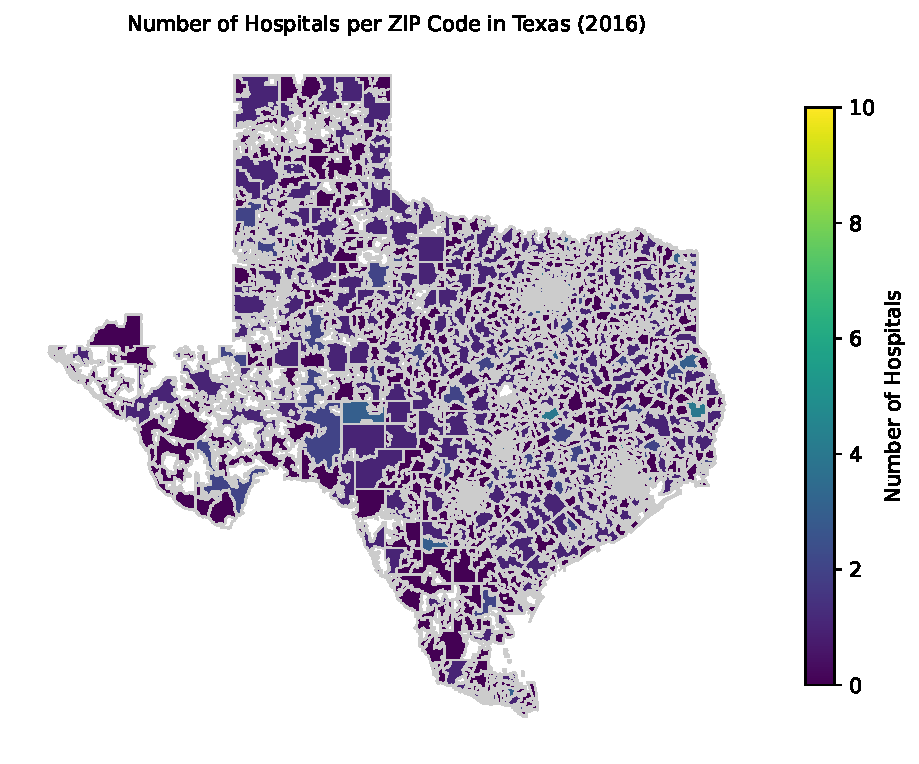
\includegraphics{pset4_template_files/figure-pdf/cell-11-output-2.pdf}

\subsection{Calculate zip code's distance to the nearest hospital (20
pts)
(*)}\label{calculate-zip-codes-distance-to-the-nearest-hospital-20-pts}

\begin{enumerate}
\def\labelenumi{\arabic{enumi}.}
\tightlist
\item
\end{enumerate}

\begin{Shaded}
\begin{Highlighting}[]
\NormalTok{base\_path }\OperatorTok{=} \StringTok{\textquotesingle{}\textasciitilde{}/Desktop/gz\_2010\_us\_860\_00\_500k\textquotesingle{}}
\NormalTok{shapefile\_path }\OperatorTok{=}\NormalTok{ os.path.join(base\_path, }\StringTok{"gz\_2010\_us\_860\_00\_500k.shp"}\NormalTok{)}

\NormalTok{gdf }\OperatorTok{=}\NormalTok{ gpd.read\_file(shapefile\_path)}

\NormalTok{zips\_all\_centroids }\OperatorTok{=}\NormalTok{ gdf.copy()}
\NormalTok{zips\_all\_centroids[}\StringTok{"geometry"}\NormalTok{] }\OperatorTok{=}\NormalTok{ gdf.centroid}

\BuiltInTok{print}\NormalTok{(}\StringTok{"GeoDataFrame dimensionality:"}\NormalTok{, zips\_all\_centroids.shape)}
\BuiltInTok{print}\NormalTok{(}\StringTok{"GeoDataFrame Column information:"}\NormalTok{)}
\BuiltInTok{print}\NormalTok{(zips\_all\_centroids.columns)}

\BuiltInTok{print}\NormalTok{(zips\_all\_centroids.head())}
\end{Highlighting}
\end{Shaded}

\begin{verbatim}
/var/folders/6t/pjbppdks0vb8q5hf3h8p6mx00000gn/T/ipykernel_27552/4045363704.py:7: UserWarning:

Geometry is in a geographic CRS. Results from 'centroid' are likely incorrect. Use 'GeoSeries.to_crs()' to re-project geometries to a projected CRS before this operation.

\end{verbatim}

\begin{verbatim}
GeoDataFrame dimensionality: (33120, 6)
GeoDataFrame Column information:
Index(['GEO_ID', 'ZCTA5', 'NAME', 'LSAD', 'CENSUSAREA', 'geometry'], dtype='object')
           GEO_ID  ZCTA5   NAME   LSAD  CENSUSAREA                    geometry
0  8600000US01040  01040  01040  ZCTA5      21.281  POINT (-72.64107 42.21257)
1  8600000US01050  01050  01050  ZCTA5      38.329  POINT (-72.86985 42.28786)
2  8600000US01053  01053  01053  ZCTA5       5.131  POINT (-72.71162 42.35349)
3  8600000US01056  01056  01056  ZCTA5      27.205  POINT (-72.45805 42.19215)
4  8600000US01057  01057  01057  ZCTA5      44.907   POINT (-72.3243 42.09165)
\end{verbatim}

\begin{enumerate}
\def\labelenumi{\arabic{enumi}.}
\setcounter{enumi}{1}
\tightlist
\item
\end{enumerate}

\begin{Shaded}
\begin{Highlighting}[]
\NormalTok{texas\_prefixes }\OperatorTok{=}\NormalTok{ (}\StringTok{"75"}\NormalTok{, }\StringTok{"76"}\NormalTok{, }\StringTok{"77"}\NormalTok{, }\StringTok{"78"}\NormalTok{, }\StringTok{"79"}\NormalTok{)}

\NormalTok{zips\_texas\_centroids }\OperatorTok{=}\NormalTok{ zips\_all\_centroids[}
\NormalTok{    zips\_all\_centroids[}\StringTok{"ZCTA5"}\NormalTok{].}\BuiltInTok{str}\NormalTok{.startswith(texas\_prefixes)}
\NormalTok{]}
\NormalTok{num\_unique\_texas\_zips }\OperatorTok{=}\NormalTok{ zips\_texas\_centroids[}\StringTok{"ZCTA5"}\NormalTok{].nunique()}
\BuiltInTok{print}\NormalTok{(}\SpecialStringTok{f"Number of unique zip codes in Texas: }\SpecialCharTok{\{}\NormalTok{num\_unique\_texas\_zips}\SpecialCharTok{\}}\SpecialStringTok{"}\NormalTok{)}

\NormalTok{bordering\_state\_prefixes }\OperatorTok{=}\NormalTok{ (}
    \StringTok{"70"}\NormalTok{,}
    \StringTok{"71"}\NormalTok{,}
    \StringTok{"72"}\NormalTok{,}
    \StringTok{"73"}\NormalTok{,}
    \StringTok{"74"}\NormalTok{,}
    \StringTok{"75"}\NormalTok{,}
    \StringTok{"76"}\NormalTok{,}
    \StringTok{"77"}\NormalTok{,}
    \StringTok{"78"}\NormalTok{,}
    \StringTok{"79"}\NormalTok{,}
    \StringTok{"87"}\NormalTok{,}
    \StringTok{"88"}\NormalTok{,}
\NormalTok{)}

\NormalTok{zips\_texas\_borderstates\_centroids }\OperatorTok{=}\NormalTok{ zips\_all\_centroids[}
\NormalTok{    zips\_all\_centroids[}\StringTok{"ZCTA5"}\NormalTok{].}\BuiltInTok{str}\NormalTok{.startswith(bordering\_state\_prefixes)}
\NormalTok{]}
\NormalTok{num\_unique\_borderstate\_zips }\OperatorTok{=}\NormalTok{ zips\_texas\_borderstates\_centroids[}\StringTok{"ZCTA5"}\NormalTok{].nunique()}
\BuiltInTok{print}\NormalTok{(}
    \SpecialStringTok{f"Number of unique zip codes in Texas and bordering states: }\SpecialCharTok{\{}\NormalTok{num\_unique\_borderstate\_zips}\SpecialCharTok{\}}\SpecialStringTok{"}
\NormalTok{)}
\end{Highlighting}
\end{Shaded}

\begin{verbatim}
Number of unique zip codes in Texas: 1935
Number of unique zip codes in Texas and bordering states: 4057
\end{verbatim}

\begin{enumerate}
\def\labelenumi{\arabic{enumi}.}
\setcounter{enumi}{2}
\tightlist
\item
\end{enumerate}

\begin{Shaded}
\begin{Highlighting}[]
\NormalTok{short\_term\_category\_code }\OperatorTok{=} \DecValTok{1}
\NormalTok{short\_term\_subtype\_code }\OperatorTok{=} \DecValTok{1}
\NormalTok{active\_code }\OperatorTok{=} \DecValTok{0}

\NormalTok{active\_hospitals\_2016 }\OperatorTok{=}\NormalTok{ pos2016[}
\NormalTok{    (pos2016[}\StringTok{\textquotesingle{}PRVDR\_CTGRY\_CD\textquotesingle{}}\NormalTok{] }\OperatorTok{==}\NormalTok{ short\_term\_category\_code) }\OperatorTok{\&}
\NormalTok{    (pos2016[}\StringTok{\textquotesingle{}PRVDR\_CTGRY\_SBTYP\_CD\textquotesingle{}}\NormalTok{] }\OperatorTok{==}\NormalTok{ short\_term\_subtype\_code) }\OperatorTok{\&}
\NormalTok{    (pos2016[}\StringTok{\textquotesingle{}PGM\_TRMNTN\_CD\textquotesingle{}}\NormalTok{] }\OperatorTok{==}\NormalTok{ active\_code)}
\NormalTok{]}

\NormalTok{active\_hospitals\_2016 }\OperatorTok{=}\NormalTok{ active\_hospitals\_2016.copy()}

\NormalTok{active\_hospitals\_2016[}\StringTok{\textquotesingle{}ZIP\_CD\textquotesingle{}}\NormalTok{] }\OperatorTok{=}\NormalTok{ active\_hospitals\_2016[}\StringTok{\textquotesingle{}ZIP\_CD\textquotesingle{}}\NormalTok{].fillna(}\DecValTok{0}\NormalTok{).astype(}\BuiltInTok{int}\NormalTok{).astype(}\BuiltInTok{str}\NormalTok{).}\BuiltInTok{str}\NormalTok{.zfill(}\DecValTok{5}\NormalTok{)}

\NormalTok{hospital\_counts }\OperatorTok{=}\NormalTok{ active\_hospitals\_2016[}\StringTok{\textquotesingle{}ZIP\_CD\textquotesingle{}}\NormalTok{].value\_counts().reset\_index()}
\NormalTok{hospital\_counts.columns }\OperatorTok{=}\NormalTok{ [}\StringTok{\textquotesingle{}ZCTA5\textquotesingle{}}\NormalTok{, }\StringTok{\textquotesingle{}hospital\_count\textquotesingle{}}\NormalTok{]}

\NormalTok{zips\_with\_hospitals }\OperatorTok{=}\NormalTok{ hospital\_counts[hospital\_counts[}\StringTok{\textquotesingle{}hospital\_count\textquotesingle{}}\NormalTok{] }\OperatorTok{\textgreater{}=} \DecValTok{1}\NormalTok{]}

\NormalTok{zips\_withhospital\_centroids }\OperatorTok{=}\NormalTok{ zips\_texas\_borderstates\_centroids.merge(}
\NormalTok{    zips\_with\_hospitals, on}\OperatorTok{=}\StringTok{\textquotesingle{}ZCTA5\textquotesingle{}}\NormalTok{, how}\OperatorTok{=}\StringTok{\textquotesingle{}inner\textquotesingle{}}
\NormalTok{)}

\BuiltInTok{print}\NormalTok{(zips\_withhospital\_centroids.head())}
\BuiltInTok{print}\NormalTok{(}\SpecialStringTok{f"Number of zip codes with at least 1 hospital in 2016: }\SpecialCharTok{\{}\NormalTok{zips\_withhospital\_centroids}\SpecialCharTok{.}\NormalTok{shape[}\DecValTok{0}\NormalTok{]}\SpecialCharTok{\}}\SpecialStringTok{"}\NormalTok{)}
\end{Highlighting}
\end{Shaded}

\begin{verbatim}
           GEO_ID  ZCTA5   NAME   LSAD  CENSUSAREA  \
0  8600000US70043  70043  70043  ZCTA5       7.775   
1  8600000US70127  70127  70127  ZCTA5       7.095   
2  8600000US70301  70301  70301  ZCTA5     288.050   
3  8600000US70360  70360  70360  ZCTA5      64.325   
4  8600000US70403  70403  70403  ZCTA5      42.960   

                     geometry  hospital_count  
0  POINT (-89.96276 29.94804)               1  
1  POINT (-89.97675 30.02501)               1  
2   POINT (-90.74089 29.8141)               1  
3  POINT (-90.81028 29.58819)               2  
4  POINT (-90.48388 30.48002)               2  
Number of zip codes with at least 1 hospital in 2016: 448
\end{verbatim}

\begin{enumerate}
\def\labelenumi{\arabic{enumi}.}
\setcounter{enumi}{3}
\tightlist
\item
  \begin{enumerate}
  \def\labelenumii{\alph{enumii}.}
  \tightlist
  \item
  \end{enumerate}
\end{enumerate}

\begin{Shaded}
\begin{Highlighting}[]
\ImportTok{import}\NormalTok{ time }

\NormalTok{zips\_texas\_centroids }\OperatorTok{=}\NormalTok{ zips\_texas\_centroids.to\_crs(epsg}\OperatorTok{=}\DecValTok{3857}\NormalTok{)}
\NormalTok{zips\_withhospital\_centroids }\OperatorTok{=}\NormalTok{ zips\_withhospital\_centroids.to\_crs(epsg}\OperatorTok{=}\DecValTok{3857}\NormalTok{)}

\NormalTok{test\_zips }\OperatorTok{=}\NormalTok{ zips\_texas\_centroids.head(}\DecValTok{10}\NormalTok{)}

\NormalTok{start\_time }\OperatorTok{=}\NormalTok{ time.time()}

\NormalTok{distances }\OperatorTok{=}\NormalTok{ []}

\ControlFlowTok{for}\NormalTok{ \_, test\_zip }\KeywordTok{in}\NormalTok{ test\_zips.iterrows():}
\NormalTok{    test\_geometry }\OperatorTok{=}\NormalTok{ test\_zip[}\StringTok{"geometry"}\NormalTok{]}

\NormalTok{    min\_distance }\OperatorTok{=}\NormalTok{ zips\_withhospital\_centroids[}\StringTok{"geometry"}\NormalTok{].distance(test\_geometry).}\BuiltInTok{min}\NormalTok{()}

\NormalTok{    distances.append(}
\NormalTok{        \{}\StringTok{"ZCTA5"}\NormalTok{: test\_zip[}\StringTok{"ZCTA5"}\NormalTok{], }\StringTok{"Nearest\_Hospital\_Distance"}\NormalTok{: min\_distance\}}
\NormalTok{    )}

\NormalTok{end\_time }\OperatorTok{=}\NormalTok{ time.time()}

\NormalTok{execution\_time }\OperatorTok{=}\NormalTok{ end\_time }\OperatorTok{{-}}\NormalTok{ start\_time}
\BuiltInTok{print}\NormalTok{(}\SpecialStringTok{f"Time taken for 10 zip codes: }\SpecialCharTok{\{}\NormalTok{execution\_time}\SpecialCharTok{:.2f\}}\SpecialStringTok{ seconds"}\NormalTok{)}

\NormalTok{distance\_results }\OperatorTok{=}\NormalTok{ pd.DataFrame(distances)}
\BuiltInTok{print}\NormalTok{(distance\_results)}

\NormalTok{total\_zip\_codes }\OperatorTok{=} \BuiltInTok{len}\NormalTok{(zips\_texas\_centroids)}
\NormalTok{estimated\_time }\OperatorTok{=}\NormalTok{ (execution\_time }\OperatorTok{/} \DecValTok{10}\NormalTok{) }\OperatorTok{*}\NormalTok{ total\_zip\_codes}
\BuiltInTok{print}\NormalTok{(}\SpecialStringTok{f"Estimated time for all zip codes in Texas: }\SpecialCharTok{\{}\NormalTok{estimated\_time }\OperatorTok{/} \DecValTok{60}\SpecialCharTok{:.2f\}}\SpecialStringTok{ minutes"}\NormalTok{)}
\end{Highlighting}
\end{Shaded}

\begin{verbatim}
Time taken for 10 zip codes: 0.00 seconds
   ZCTA5  Nearest_Hospital_Distance
0  78624                   0.000000
1  78626               21443.710461
2  78628               14228.011802
3  78631               42374.908087
4  78632               28125.820177
5  78633               27182.105800
6  78634               13251.123905
7  78635               36496.178533
8  78636               41783.476410
9  78638               22509.393995
Estimated time for all zip codes in Texas: 0.01 minutes
\end{verbatim}

\begin{verbatim}
b.
\end{verbatim}

\begin{Shaded}
\begin{Highlighting}[]
\NormalTok{start\_time }\OperatorTok{=}\NormalTok{ time.time()}

\NormalTok{all\_distances }\OperatorTok{=}\NormalTok{ []}

\ControlFlowTok{for}\NormalTok{ \_, texas\_zip }\KeywordTok{in}\NormalTok{ zips\_texas\_centroids.iterrows():}
\NormalTok{    texas\_geometry }\OperatorTok{=}\NormalTok{ texas\_zip[}\StringTok{"geometry"}\NormalTok{]}

\NormalTok{    min\_distance }\OperatorTok{=}\NormalTok{ (}
\NormalTok{        zips\_withhospital\_centroids[}\StringTok{"geometry"}\NormalTok{].distance(texas\_geometry).}\BuiltInTok{min}\NormalTok{()}
\NormalTok{    )}

\NormalTok{    all\_distances.append(}
\NormalTok{        \{}\StringTok{"ZCTA5"}\NormalTok{: texas\_zip[}\StringTok{"ZCTA5"}\NormalTok{], }\StringTok{"Nearest\_Hospital\_Distance"}\NormalTok{: min\_distance\}}
\NormalTok{    )}

\NormalTok{end\_time }\OperatorTok{=}\NormalTok{ time.time()}

\NormalTok{execution\_time }\OperatorTok{=}\NormalTok{ end\_time }\OperatorTok{{-}}\NormalTok{ start\_time}
\BuiltInTok{print}\NormalTok{(}\SpecialStringTok{f"Time taken for all zip codes in Texas: }\SpecialCharTok{\{}\NormalTok{execution\_time}\SpecialCharTok{:.2f\}}\SpecialStringTok{ seconds"}\NormalTok{)}

\NormalTok{all\_distance\_results }\OperatorTok{=}\NormalTok{ pd.DataFrame(all\_distances)}
\BuiltInTok{print}\NormalTok{(all\_distance\_results.head())}

\NormalTok{all\_distance\_results.to\_csv(}\StringTok{"texas\_zipcode\_hospital\_distances.csv"}\NormalTok{, index}\OperatorTok{=}\VariableTok{False}\NormalTok{)}

\NormalTok{estimated\_time }\OperatorTok{=}\NormalTok{ (}\FloatTok{0.08} \OperatorTok{/} \DecValTok{10}\NormalTok{) }\OperatorTok{*} \BuiltInTok{len}\NormalTok{(zips\_texas\_centroids)}
\BuiltInTok{print}\NormalTok{(}\SpecialStringTok{f"Estimated time for all zip codes in Texas: }\SpecialCharTok{\{}\NormalTok{estimated\_time}\SpecialCharTok{:.2f\}}\SpecialStringTok{ seconds"}\NormalTok{)}

\ControlFlowTok{if}\NormalTok{ execution\_time }\OperatorTok{\textless{}=}\NormalTok{ estimated\_time:}
    \BuiltInTok{print}\NormalTok{(}\StringTok{"Actual execution time is less than or close to the estimated time."}\NormalTok{)}
\ControlFlowTok{else}\NormalTok{:}
    \BuiltInTok{print}\NormalTok{(}\StringTok{"Actual execution time is greater than the estimated time."}\NormalTok{)}
\end{Highlighting}
\end{Shaded}

\begin{verbatim}
Time taken for all zip codes in Texas: 0.31 seconds
   ZCTA5  Nearest_Hospital_Distance
0  78624                   0.000000
1  78626               21443.710461
2  78628               14228.011802
3  78631               42374.908087
4  78632               28125.820177
Estimated time for all zip codes in Texas: 15.48 seconds
Actual execution time is less than or close to the estimated time.
\end{verbatim}

\begin{enumerate}
\def\labelenumi{\arabic{enumi}.}
\setcounter{enumi}{4}
\item
  \begin{enumerate}
  \def\labelenumii{\alph{enumii}.}
  \item
    \#\#\# Ans: The unit in the .prj file is Degree.
  \item
  \end{enumerate}
\end{enumerate}

\begin{Shaded}
\begin{Highlighting}[]
\NormalTok{conversion\_factor }\OperatorTok{=} \FloatTok{0.000621371}

\NormalTok{all\_distance\_results[}\StringTok{"Nearest\_Hospital\_Distance\_Miles"}\NormalTok{] }\OperatorTok{=}\NormalTok{ (}
\NormalTok{    all\_distance\_results[}\StringTok{"Nearest\_Hospital\_Distance"}\NormalTok{] }\OperatorTok{*}\NormalTok{ conversion\_factor}
\NormalTok{)}

\NormalTok{average\_distance\_miles }\OperatorTok{=}\NormalTok{ all\_distance\_results[}\StringTok{"Nearest\_Hospital\_Distance\_Miles"}\NormalTok{].mean()}
\BuiltInTok{print}\NormalTok{(}
    \SpecialStringTok{f"Average distance to the nearest hospital in Texas (in miles): }\SpecialCharTok{\{}\NormalTok{average\_distance\_miles}\SpecialCharTok{:.2f\}}\SpecialStringTok{ miles"}
\NormalTok{)}

\ControlFlowTok{if}\NormalTok{ average\_distance\_miles }\OperatorTok{\textless{}} \DecValTok{30}\NormalTok{:}
    \BuiltInTok{print}\NormalTok{(}
        \StringTok{"This value makes sense, considering the distribution of hospitals and rural areas in Texas."}
\NormalTok{    )}
\ControlFlowTok{else}\NormalTok{:}
    \BuiltInTok{print}\NormalTok{(}
        \StringTok{"This value seems unusually high, possibly indicating a lack of hospitals in some areas."}
\NormalTok{    )}
\end{Highlighting}
\end{Shaded}

\begin{verbatim}
Average distance to the nearest hospital in Texas (in miles): 15.77 miles
This value makes sense, considering the distribution of hospitals and rural areas in Texas.
\end{verbatim}

\begin{verbatim}
c.
\end{verbatim}

\begin{Shaded}
\begin{Highlighting}[]
\NormalTok{base\_path }\OperatorTok{=} \StringTok{"/Users/cynthia/Desktop/gz\_2010\_us\_860\_00\_500k"}
\NormalTok{pathshp }\OperatorTok{=}\NormalTok{ os.path.join(base\_path, }\StringTok{"gz\_2010\_us\_860\_00\_500k.shp"}\NormalTok{)}
\NormalTok{df\_shp }\OperatorTok{=}\NormalTok{ gpd.read\_file(pathshp)}

\NormalTok{df\_texas }\OperatorTok{=}\NormalTok{ df\_shp[df\_shp[}\StringTok{"ZCTA5"}\NormalTok{].}\BuiltInTok{str}\NormalTok{.startswith((}\StringTok{"75"}\NormalTok{, }\StringTok{"76"}\NormalTok{, }\StringTok{"77"}\NormalTok{, }\StringTok{"78"}\NormalTok{, }\StringTok{"79"}\NormalTok{))]}
\NormalTok{df\_texas[}\StringTok{"ZCTA5"}\NormalTok{] }\OperatorTok{=}\NormalTok{ df\_texas[}\StringTok{"ZCTA5"}\NormalTok{].astype(}\BuiltInTok{str}\NormalTok{)}

\NormalTok{df\_texas\_distance }\OperatorTok{=}\NormalTok{ df\_texas.merge(}
\NormalTok{    all\_distance\_results[[}\StringTok{"ZCTA5"}\NormalTok{, }\StringTok{"Nearest\_Hospital\_Distance\_Miles"}\NormalTok{]],}
\NormalTok{    on}\OperatorTok{=}\StringTok{"ZCTA5"}\NormalTok{,}
\NormalTok{    how}\OperatorTok{=}\StringTok{"left"}
\NormalTok{)}

\NormalTok{df\_texas\_distance[}\StringTok{"Nearest\_Hospital\_Distance\_Miles"}\NormalTok{] }\OperatorTok{=}\NormalTok{ df\_texas\_distance[}\StringTok{"Nearest\_Hospital\_Distance\_Miles"}\NormalTok{].fillna(}\DecValTok{0}\NormalTok{)}

\NormalTok{fig, ax }\OperatorTok{=}\NormalTok{ plt.subplots(}\DecValTok{1}\NormalTok{, }\DecValTok{1}\NormalTok{, figsize}\OperatorTok{=}\NormalTok{(}\DecValTok{8}\NormalTok{, }\DecValTok{10}\NormalTok{))}
\NormalTok{df\_texas\_distance.plot(}
\NormalTok{    column}\OperatorTok{=}\StringTok{"Nearest\_Hospital\_Distance\_Miles"}\NormalTok{,}
\NormalTok{    cmap}\OperatorTok{=}\StringTok{"OrRd"}\NormalTok{,}
\NormalTok{    linewidth}\OperatorTok{=}\FloatTok{0.8}\NormalTok{,}
\NormalTok{    ax}\OperatorTok{=}\NormalTok{ax,}
\NormalTok{    edgecolor}\OperatorTok{=}\StringTok{"0.8"}\NormalTok{,}
\NormalTok{    legend}\OperatorTok{=}\VariableTok{True}\NormalTok{,}
\NormalTok{    legend\_kwds}\OperatorTok{=}\NormalTok{\{}
        \StringTok{\textquotesingle{}shrink\textquotesingle{}}\NormalTok{: }\FloatTok{0.5}\NormalTok{,  }
        \StringTok{\textquotesingle{}label\textquotesingle{}}\NormalTok{: }\StringTok{"Distance (miles)"} 
\NormalTok{    \},}
\NormalTok{)}

\NormalTok{ax.set\_title(}\StringTok{"Distance to Nearest Hospital by Zip Code in Texas (in Miles)"}\NormalTok{, fontsize}\OperatorTok{=}\DecValTok{10}\NormalTok{)}
\NormalTok{plt.axis(}\StringTok{"off"}\NormalTok{)}

\NormalTok{plt.show()}
\end{Highlighting}
\end{Shaded}

\begin{verbatim}
/opt/anaconda3/lib/python3.11/site-packages/geopandas/geodataframe.py:1819: SettingWithCopyWarning:


A value is trying to be set on a copy of a slice from a DataFrame.
Try using .loc[row_indexer,col_indexer] = value instead

See the caveats in the documentation: https://pandas.pydata.org/pandas-docs/stable/user_guide/indexing.html#returning-a-view-versus-a-copy
\end{verbatim}

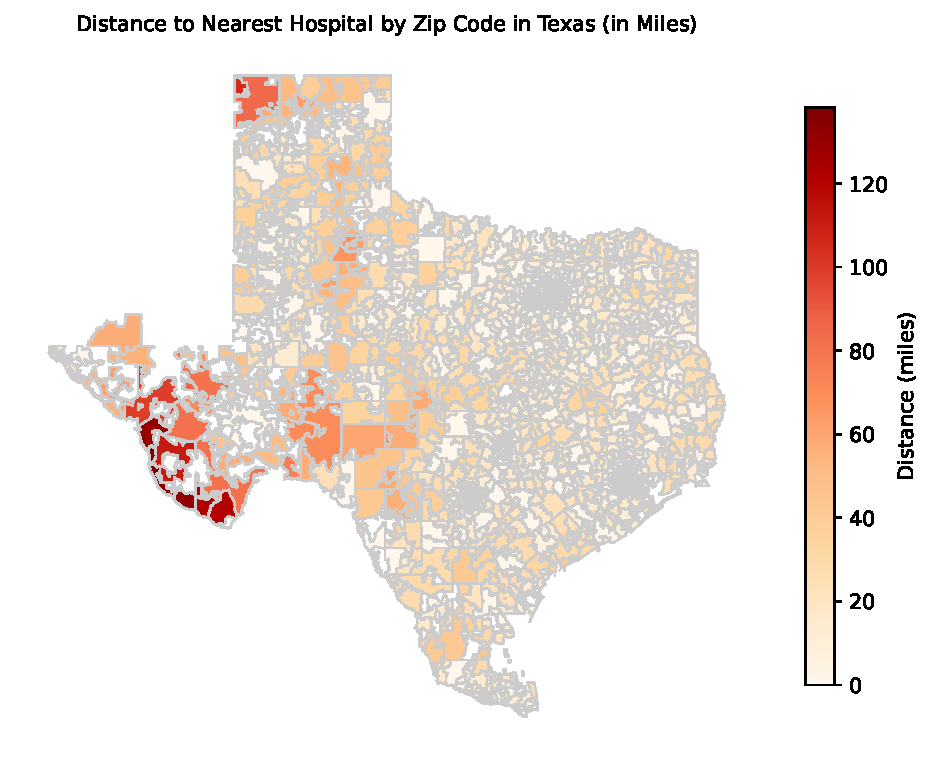
\includegraphics{pset4_template_files/figure-pdf/cell-18-output-2.pdf}

\subsection{Effects of closures on access in Texas (15
pts)}\label{effects-of-closures-on-access-in-texas-15-pts}

\begin{enumerate}
\def\labelenumi{\arabic{enumi}.}
\tightlist
\item
\end{enumerate}

\begin{Shaded}
\begin{Highlighting}[]
\NormalTok{columns\_to\_drop }\OperatorTok{=}\NormalTok{ [}
\NormalTok{    col }\ControlFlowTok{for}\NormalTok{ col }\KeywordTok{in}\NormalTok{ filtered\_suspected\_closures\_df.columns }\ControlFlowTok{if} \StringTok{\textquotesingle{}STATE\_CD\textquotesingle{}} \KeywordTok{in}\NormalTok{ col]}
\NormalTok{filtered\_suspected\_closures\_df }\OperatorTok{=}\NormalTok{ filtered\_suspected\_closures\_df.drop(}
\NormalTok{    columns}\OperatorTok{=}\NormalTok{columns\_to\_drop, errors}\OperatorTok{=}\StringTok{\textquotesingle{}ignore\textquotesingle{}}\NormalTok{)}

\NormalTok{filtered\_suspected\_closures\_df }\OperatorTok{=}\NormalTok{ filtered\_suspected\_closures\_df.merge(}
\NormalTok{    dataframes[}\DecValTok{0}\NormalTok{][[}\StringTok{\textquotesingle{}PRVDR\_NUM\textquotesingle{}}\NormalTok{, }\StringTok{\textquotesingle{}STATE\_CD\textquotesingle{}}\NormalTok{]],}
\NormalTok{    on}\OperatorTok{=}\StringTok{\textquotesingle{}PRVDR\_NUM\textquotesingle{}}\NormalTok{,}
\NormalTok{    how}\OperatorTok{=}\StringTok{\textquotesingle{}left\textquotesingle{}}
\NormalTok{)}

\NormalTok{state\_column }\OperatorTok{=} \StringTok{\textquotesingle{}STATE\_CD\textquotesingle{}}
\NormalTok{texas\_closures\_df }\OperatorTok{=}\NormalTok{ filtered\_suspected\_closures\_df[filtered\_suspected\_closures\_df[state\_column] }\OperatorTok{==} \StringTok{\textquotesingle{}TX\textquotesingle{}}\NormalTok{].copy(}
\NormalTok{)}

\NormalTok{texas\_closures\_df[}\StringTok{\textquotesingle{}ZIP Code\textquotesingle{}}\NormalTok{] }\OperatorTok{=}\NormalTok{ texas\_closures\_df[}\StringTok{\textquotesingle{}ZIP Code\textquotesingle{}}\NormalTok{].astype(}
    \BuiltInTok{str}\NormalTok{).}\BuiltInTok{str}\NormalTok{.zfill(}\DecValTok{5}\NormalTok{)}

\NormalTok{closures\_per\_zip }\OperatorTok{=}\NormalTok{ texas\_closures\_df.groupby(}
    \StringTok{\textquotesingle{}ZIP Code\textquotesingle{}}\NormalTok{).size().reset\_index(name}\OperatorTok{=}\StringTok{\textquotesingle{}closure\_count\textquotesingle{}}\NormalTok{)}
\NormalTok{closures\_per\_zip }\OperatorTok{=}\NormalTok{ closures\_per\_zip.rename(columns}\OperatorTok{=}\NormalTok{\{}\StringTok{"ZIP Code"}\NormalTok{: }\StringTok{"ZIP\_CD"}\NormalTok{\})}

\NormalTok{closures\_per\_zip[}\StringTok{\textquotesingle{}ZIP\_CD\textquotesingle{}}\NormalTok{] }\OperatorTok{=}\NormalTok{ closures\_per\_zip[}\StringTok{\textquotesingle{}ZIP\_CD\textquotesingle{}}\NormalTok{].astype(}
    \BuiltInTok{str}\NormalTok{).}\BuiltInTok{str}\NormalTok{.replace(}\VerbatimStringTok{r\textquotesingle{}\textbackslash{}.0$\textquotesingle{}}\NormalTok{, }\StringTok{\textquotesingle{}\textquotesingle{}}\NormalTok{, regex}\OperatorTok{=}\VariableTok{True}\NormalTok{).}\BuiltInTok{str}\NormalTok{.zfill(}\DecValTok{5}\NormalTok{)}

\NormalTok{closures\_per\_zip }\OperatorTok{=}\NormalTok{ closures\_per\_zip.sort\_values(by}\OperatorTok{=}\StringTok{\textquotesingle{}ZIP\_CD\textquotesingle{}}\NormalTok{)}

\NormalTok{closures\_per\_zip.reset\_index(inplace}\OperatorTok{=}\VariableTok{True}\NormalTok{)}
\NormalTok{closures\_per\_zip.rename(columns}\OperatorTok{=}\NormalTok{\{}\StringTok{"index"}\NormalTok{: }\StringTok{" "}\NormalTok{\}, inplace}\OperatorTok{=}\VariableTok{True}\NormalTok{)}

\BuiltInTok{print}\NormalTok{(closures\_per\_zip.to\_string(index}\OperatorTok{=}\VariableTok{False}\NormalTok{))}
\end{Highlighting}
\end{Shaded}

\begin{verbatim}
   ZIP_CD  closure_count
 0  75051              1
 1  75087              1
 2  75140              1
 3  75235              1
 4  75390              1
 5  76520              1
 6  76531              1
 7  76645              1
 8  77065              1
 9  78336              1
10  78613              1
11  79520              1
12  79529              1
13  79902              1
\end{verbatim}

\begin{enumerate}
\def\labelenumi{\arabic{enumi}.}
\setcounter{enumi}{1}
\tightlist
\item
\end{enumerate}

\begin{Shaded}
\begin{Highlighting}[]
\NormalTok{df\_texas }\OperatorTok{=}\NormalTok{ df\_shp[df\_shp[}\StringTok{"ZCTA5"}\NormalTok{].}\BuiltInTok{str}\NormalTok{.startswith(}
\NormalTok{    (}\StringTok{"75"}\NormalTok{, }\StringTok{"76"}\NormalTok{, }\StringTok{"77"}\NormalTok{, }\StringTok{"78"}\NormalTok{, }\StringTok{"79"}\NormalTok{))].copy()}

\NormalTok{df\_texas[}\StringTok{\textquotesingle{}ZCTA5\textquotesingle{}}\NormalTok{] }\OperatorTok{=}\NormalTok{ df\_texas[}\StringTok{\textquotesingle{}ZCTA5\textquotesingle{}}\NormalTok{].astype(}\BuiltInTok{str}\NormalTok{).}\BuiltInTok{str}\NormalTok{.zfill(}\DecValTok{5}\NormalTok{)}

\NormalTok{closures\_per\_zip[}\StringTok{\textquotesingle{}ZIP\_CD\textquotesingle{}}\NormalTok{] }\OperatorTok{=}\NormalTok{ closures\_per\_zip[}\StringTok{\textquotesingle{}ZIP\_CD\textquotesingle{}}\NormalTok{].astype(}
    \BuiltInTok{str}\NormalTok{).}\BuiltInTok{str}\NormalTok{.zfill(}\DecValTok{5}\NormalTok{)}

\NormalTok{map\_closures\_texas }\OperatorTok{=}\NormalTok{ df\_texas.merge(}
\NormalTok{    closures\_per\_zip, left\_on}\OperatorTok{=}\StringTok{\textquotesingle{}ZCTA5\textquotesingle{}}\NormalTok{, right\_on}\OperatorTok{=}\StringTok{\textquotesingle{}ZIP\_CD\textquotesingle{}}\NormalTok{, how}\OperatorTok{=}\StringTok{\textquotesingle{}left\textquotesingle{}}
\NormalTok{)}
\NormalTok{map\_closures\_texas[}\StringTok{\textquotesingle{}closure\_count\textquotesingle{}}\NormalTok{] }\OperatorTok{=}\NormalTok{ map\_closures\_texas[}\StringTok{\textquotesingle{}closure\_count\textquotesingle{}}\NormalTok{].fillna(}
    \DecValTok{0}\NormalTok{)}

\NormalTok{fig, ax }\OperatorTok{=}\NormalTok{ plt.subplots(}\DecValTok{1}\NormalTok{, }\DecValTok{1}\NormalTok{, figsize}\OperatorTok{=}\NormalTok{(}\DecValTok{8}\NormalTok{, }\DecValTok{10}\NormalTok{))}
\NormalTok{map\_closures\_texas.plot(}
\NormalTok{    column}\OperatorTok{=}\StringTok{\textquotesingle{}closure\_count\textquotesingle{}}\NormalTok{,}
\NormalTok{    cmap}\OperatorTok{=}\StringTok{\textquotesingle{}Reds\textquotesingle{}}\NormalTok{,}
\NormalTok{    legend}\OperatorTok{=}\VariableTok{True}\NormalTok{,}
\NormalTok{    ax}\OperatorTok{=}\NormalTok{ax,}
\NormalTok{    linewidth}\OperatorTok{=}\FloatTok{0.8}\NormalTok{,}
\NormalTok{    edgecolor}\OperatorTok{=}\StringTok{\textquotesingle{}0.8\textquotesingle{}}\NormalTok{,}
\NormalTok{    legend\_kwds}\OperatorTok{=}\NormalTok{\{}
        \StringTok{\textquotesingle{}shrink\textquotesingle{}}\NormalTok{: }\FloatTok{0.5}\NormalTok{, }
\NormalTok{    \}}
\NormalTok{)}
\NormalTok{ax.set\_axis\_off()}
\NormalTok{plt.title(}\StringTok{\textquotesingle{}Texas Zip Codes Affected by Hospital Closures (2016{-}2019)\textquotesingle{}}\NormalTok{, fontsize}\OperatorTok{=}\DecValTok{10}\NormalTok{)}
\NormalTok{plt.show()}


\NormalTok{directly\_zip\_count }\OperatorTok{=}\NormalTok{ closures\_per\_zip.shape[}\DecValTok{0}\NormalTok{]}
\BuiltInTok{print}\NormalTok{(}
    \SpecialStringTok{f"The number of directly affected zip codes in Texas is }\SpecialCharTok{\{}\NormalTok{directly\_zip\_count}\SpecialCharTok{\}}\SpecialStringTok{."}\NormalTok{)}
\end{Highlighting}
\end{Shaded}

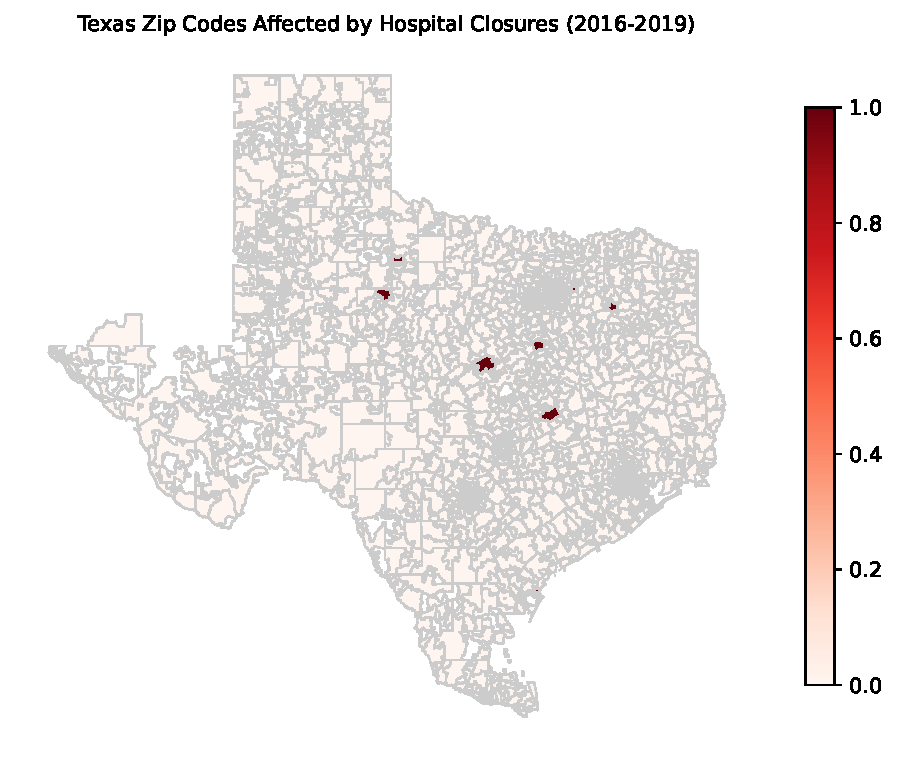
\includegraphics{pset4_template_files/figure-pdf/cell-20-output-1.pdf}

\begin{verbatim}
The number of directly affected zip codes in Texas is 14.
\end{verbatim}

\begin{enumerate}
\def\labelenumi{\arabic{enumi}.}
\setcounter{enumi}{2}
\tightlist
\item
\end{enumerate}

\begin{Shaded}
\begin{Highlighting}[]
\NormalTok{direct\_closures\_texas\_gdf }\OperatorTok{=}\NormalTok{ df\_texas.merge(}
\NormalTok{    closures\_per\_zip, left\_on}\OperatorTok{=}\StringTok{\textquotesingle{}ZCTA5\textquotesingle{}}\NormalTok{, right\_on}\OperatorTok{=}\StringTok{\textquotesingle{}ZIP\_CD\textquotesingle{}}\NormalTok{, how}\OperatorTok{=}\StringTok{\textquotesingle{}inner\textquotesingle{}}
\NormalTok{)}

\NormalTok{direct\_closures\_texas\_gdf }\OperatorTok{=}\NormalTok{ direct\_closures\_texas\_gdf.to\_crs(epsg}\OperatorTok{=}\DecValTok{3395}\NormalTok{)}

\NormalTok{closures\_buffer }\OperatorTok{=}\NormalTok{ direct\_closures\_texas\_gdf.copy()}
\NormalTok{closures\_buffer[}\StringTok{\textquotesingle{}geometry\textquotesingle{}}\NormalTok{] }\OperatorTok{=}\NormalTok{ closures\_buffer.geometry.}\BuiltInTok{buffer}\NormalTok{(}\DecValTok{16093}\NormalTok{)}

\NormalTok{closures\_buffer }\OperatorTok{=}\NormalTok{ closures\_buffer.to\_crs(df\_texas.crs)}

\NormalTok{indirectly\_zip }\OperatorTok{=}\NormalTok{ gpd.sjoin(df\_texas, closures\_buffer,}
\NormalTok{                           how}\OperatorTok{=}\StringTok{"inner"}\NormalTok{, predicate}\OperatorTok{=}\StringTok{"intersects"}\NormalTok{)}

\NormalTok{indirectly\_zip }\OperatorTok{=}\NormalTok{ indirectly\_zip[}\OperatorTok{\textasciitilde{}}\NormalTok{indirectly\_zip[}\StringTok{\textquotesingle{}ZCTA5\_left\textquotesingle{}}\NormalTok{].isin(}
\NormalTok{    direct\_closures\_texas\_gdf.to\_crs(df\_texas.crs)[}\StringTok{\textquotesingle{}ZCTA5\textquotesingle{}}\NormalTok{])]}

\NormalTok{indirectly\_zip\_count }\OperatorTok{=}\NormalTok{ indirectly\_zip[}\StringTok{\textquotesingle{}ZCTA5\_left\textquotesingle{}}\NormalTok{].nunique()}
\BuiltInTok{print}\NormalTok{(}
    \SpecialStringTok{f"The number of indirectly affected zip codes in Texas is }\SpecialCharTok{\{}\NormalTok{indirectly\_zip\_count}\SpecialCharTok{\}}\SpecialStringTok{."}\NormalTok{)}
\end{Highlighting}
\end{Shaded}

\begin{verbatim}
The number of indirectly affected zip codes in Texas is 311.
\end{verbatim}

\begin{enumerate}
\def\labelenumi{\arabic{enumi}.}
\setcounter{enumi}{3}
\tightlist
\item
\end{enumerate}

\begin{Shaded}
\begin{Highlighting}[]
\NormalTok{df\_texas[}\StringTok{\textquotesingle{}category\textquotesingle{}}\NormalTok{] }\OperatorTok{=} \StringTok{\textquotesingle{}Not Affected\textquotesingle{}}
\NormalTok{df\_texas.loc[df\_texas[}\StringTok{\textquotesingle{}ZCTA5\textquotesingle{}}\NormalTok{].isin(direct\_closures\_texas\_gdf.to\_crs(}
\NormalTok{    df\_texas.crs)[}\StringTok{\textquotesingle{}ZCTA5\textquotesingle{}}\NormalTok{]), }\StringTok{\textquotesingle{}category\textquotesingle{}}\NormalTok{] }\OperatorTok{=} \StringTok{\textquotesingle{}Directly Affected\textquotesingle{}}
\NormalTok{df\_texas.loc[df\_texas[}\StringTok{\textquotesingle{}ZCTA5\textquotesingle{}}\NormalTok{].isin(}
\NormalTok{    indirectly\_zip[}\StringTok{\textquotesingle{}ZCTA5\_left\textquotesingle{}}\NormalTok{]), }\StringTok{\textquotesingle{}category\textquotesingle{}}\NormalTok{] }\OperatorTok{=} \StringTok{\textquotesingle{}Indirectly Affected\textquotesingle{}}

\NormalTok{fig, ax }\OperatorTok{=}\NormalTok{ plt.subplots(}\DecValTok{1}\NormalTok{, }\DecValTok{1}\NormalTok{, figsize}\OperatorTok{=}\NormalTok{(}\DecValTok{8}\NormalTok{, }\DecValTok{10}\NormalTok{))}
\NormalTok{df\_texas.plot(column}\OperatorTok{=}\StringTok{\textquotesingle{}category\textquotesingle{}}\NormalTok{, ax}\OperatorTok{=}\NormalTok{ax, legend}\OperatorTok{=}\VariableTok{True}\NormalTok{,}
\NormalTok{              cmap}\OperatorTok{=}\StringTok{\textquotesingle{}Set1\textquotesingle{}}\NormalTok{, linewidth}\OperatorTok{=}\FloatTok{0.8}\NormalTok{, edgecolor}\OperatorTok{=}\StringTok{\textquotesingle{}0.8\textquotesingle{}}\NormalTok{)}
\NormalTok{plt.title(}\StringTok{\textquotesingle{}Texas Zip Codes Affected by Hospital Closures (2016{-}2019)\textquotesingle{}}\NormalTok{, fontsize}\OperatorTok{=}\DecValTok{10}\NormalTok{)}
\NormalTok{plt.axis(}\StringTok{\textquotesingle{}off\textquotesingle{}}\NormalTok{)}
\NormalTok{plt.show()}
\end{Highlighting}
\end{Shaded}

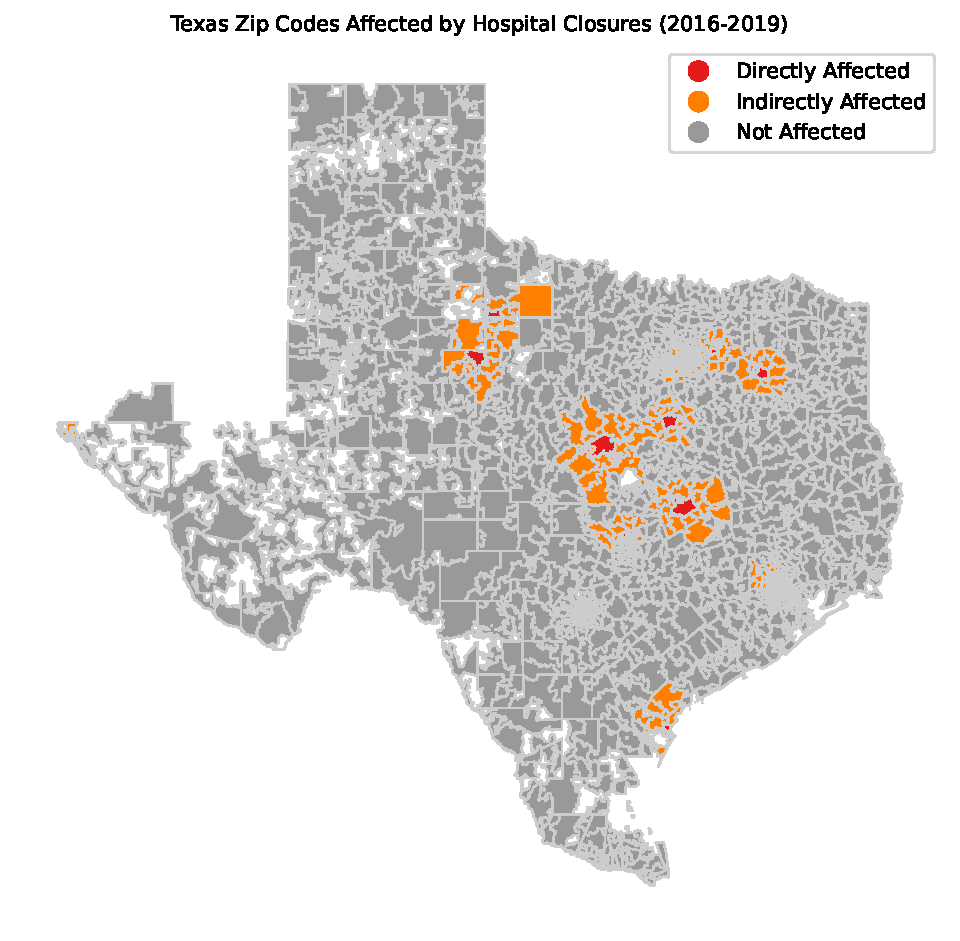
\includegraphics{pset4_template_files/figure-pdf/cell-22-output-1.pdf}

\subsection{Reflecting on the exercise (10
pts)}\label{reflecting-on-the-exercise-10-pts}

\subsection{Partner 1: The initial method for identifying hospital
closures has several problems that could lead to mistakes. One issue is
that mergers or acquisitions might be wrongly marked as closures.
Hospitals that merge or are bought may get new certification numbers,
which could make it seem like they closed. To improve accuracy, we could
better match hospital names and addresses to identify these cases.
Another issue is data delays or inconsistencies so hospitals might
temporarily disappear from the data without actually closing. Using
additional data sources, like state databases, could help verify if a
hospital is really closed. Relying on just one field, such as the
``Termination Code,'' can also be risky, because errors in that field
could lead to wrong conclusions. It would be better to also consider
other information, like staffing levels or available services. Some
hospitals may also relocate rather than close, which could be
misinterpreted as a closure. Using location data to track these changes
could help. Finally, verifying closures using official sources would
reduce false positives and make the analysis more
reliable.}\label{partner-1-the-initial-method-for-identifying-hospital-closures-has-several-problems-that-could-lead-to-mistakes.-one-issue-is-that-mergers-or-acquisitions-might-be-wrongly-marked-as-closures.-hospitals-that-merge-or-are-bought-may-get-new-certification-numbers-which-could-make-it-seem-like-they-closed.-to-improve-accuracy-we-could-better-match-hospital-names-and-addresses-to-identify-these-cases.-another-issue-is-data-delays-or-inconsistencies-so-hospitals-might-temporarily-disappear-from-the-data-without-actually-closing.-using-additional-data-sources-like-state-databases-could-help-verify-if-a-hospital-is-really-closed.-relying-on-just-one-field-such-as-the-termination-code-can-also-be-risky-because-errors-in-that-field-could-lead-to-wrong-conclusions.-it-would-be-better-to-also-consider-other-information-like-staffing-levels-or-available-services.-some-hospitals-may-also-relocate-rather-than-close-which-could-be-misinterpreted-as-a-closure.-using-location-data-to-track-these-changes-could-help.-finally-verifying-closures-using-official-sources-would-reduce-false-positives-and-make-the-analysis-more-reliable.}

\subsection{Partner 2: The current way of identifying zip codes affected
by hospital closures has some limitations. Just using distance to decide
if a zip code is directly or indirectly affected may not fully capture
changes in access to healthcare. For example, two zip codes within 10
miles of a closed hospital might be affected differently depending on
factors like transportation options, population density, and nearby
healthcare facilities. Using only distance doesn't tell the whole story.
There are some ways to improve this measure. First, include
transportation factors like road access and public transit, because
these influence how easily people can get to hospitals. Second, consider
the capacity of nearby hospitals to handle more patients, as closures
might lead to overcrowding. Third, include population density and
demographics to understand which areas might be impacted the most. Also,
consider travel time cause it can provide a better sense of
accessibility, especially in rural areas. Finally, take into account
other healthcare facilities like clinic centers to get a more complete
picture of healthcare availability after a hospital
closure.}\label{partner-2-the-current-way-of-identifying-zip-codes-affected-by-hospital-closures-has-some-limitations.-just-using-distance-to-decide-if-a-zip-code-is-directly-or-indirectly-affected-may-not-fully-capture-changes-in-access-to-healthcare.-for-example-two-zip-codes-within-10-miles-of-a-closed-hospital-might-be-affected-differently-depending-on-factors-like-transportation-options-population-density-and-nearby-healthcare-facilities.-using-only-distance-doesnt-tell-the-whole-story.-there-are-some-ways-to-improve-this-measure.-first-include-transportation-factors-like-road-access-and-public-transit-because-these-influence-how-easily-people-can-get-to-hospitals.-second-consider-the-capacity-of-nearby-hospitals-to-handle-more-patients-as-closures-might-lead-to-overcrowding.-third-include-population-density-and-demographics-to-understand-which-areas-might-be-impacted-the-most.-also-consider-travel-time-cause-it-can-provide-a-better-sense-of-accessibility-especially-in-rural-areas.-finally-take-into-account-other-healthcare-facilities-like-clinic-centers-to-get-a-more-complete-picture-of-healthcare-availability-after-a-hospital-closure.}




\end{document}
